\documentclass{beamer}
\usepackage{graphicx}
\usepackage{tikz}
\usetikzlibrary{shapes,arrows}
\usepackage{tikz}
\usetheme{default}
%\usecolortheme{seahorse}
\usepackage{default}

  \setbeamertemplate{footline}[page number]
\setbeamertemplate{navigation symbols}{}
\setbeamertemplate{frametitle}[default][center]
\setbeamerfont{frametitle}{shape=\scshape}

\usepackage{color}

{\title{\textsc{Numerical Methods-Lecture VI: Applying Newton's Method}}
\author{Trevor Gallen}
\date{}

\begin{document}


\begin{frame}
\titlepage
\end{frame}

\begin{frame}
\frametitle[alignment=center]{Motivation}
\begin{itemize}
\item We've seen the theory behind Newton's Method
\bigskip
\item How can we apply it to Value Function Iteration?
\bigskip
\begin{itemize}
\item Solving systems of equations
\bigskip
\item Maximization!
\bigskip
\item Caveat:  we'll linearly interpolate for now.
\end{itemize}
\end{itemize}
\end{frame}

\begin{frame}
\frametitle[alignment=center]{Monopolistic Competition-I}
\scriptsize
We might have a system of equations describing agent behavior.  Given elasticity of substitution $\sigma$, Income $I$, marginal cost of production $\phi$, and fixed cost of entry $\nu$, a monopolistically competitive system's equilibrium is given by: \bigskip
\begin{itemize}
\item Consumption aggregation
\begin{equation}C=\left(\int_0^nc_i^\frac{\sigma-1}{\sigma}di\right)^\frac{\sigma}{\sigma-1}\end{equation}
\item Idiosyncratic demand curves:
\begin{equation}c_i=\frac{Ip_i^{-\sigma}}{\int_0^np_i^{1-\sigma}di}\end{equation}
\item Aggregate price:
\begin{equation}P=\int_0^n\left(p_i^{1-\sigma}di\right)^\frac{1}{1-\sigma}\end{equation}
\item Profit definition:
\begin{equation}\pi_i = p_ic_i-\phi c_i - \nu\end{equation}
\item Zero profit (free entry):
\begin{equation}\pi_i=0\end{equation}
\item Optimal markup:
\begin{equation}p_i=\frac{\sigma}{\sigma-1}\phi\end{equation}
\end{itemize}
\end{frame}

\begin{frame}
\frametitle[alignment=center]{Monopolistic Competition-II}
\begin{itemize}
\bigskip
\item We won't bother simplifying, though we can in this case.
\bigskip
\item We want to solve these six equations as a function of $n,p_i,P,c_i,C,\pi_i$, and we'll assume a symmetric equilibrium.
\bigskip
\item To solve, we'll:
\bigskip
\begin{itemize}
\item Step 1:  Write all FOC's as a vectorized function of those six variables
\bigskip
\item Step 2:  Write the Jacobian of the vector of FOC's as a function of those six variables
\bigskip
\item Step 3:  Apply Newton's Method until we converge
\end{itemize}
\end{itemize}
\end{frame}


\begin{frame}
\frametitle[alignment=center]{Monopolistic Competition-III}
For code, see Lecture\_6\_NewtonsMethod\_DixitStiglitz.m
\end{frame}

%\begin{frame}
%\frametitle[alignment=center]{Motivation}
%\begin{itemize}
%\item We have Bellman Equation:
%\bigskip
%$$V(k_t)=\underset{\max}{k_{t+1}}\left\{\log(k_t^{0.7}+(1-\delta)k_t-k_{t+1})+\beta V(k_{t+1})\right\}$$
%\bigskip
%\item In other words, for a bunch of different $k$, we want to maximize:
%\bigskip
%$$F(k_{t+1};k_t)=\log(k_t^{0.7}+(1-\delta)k_t-k_{t+1})+\beta V(k_{t+1})$$
%\bigskip
%Through our choice of $k_{t+1}$.  
%\bigskip
%\item From some starting guess of $k_{t+1}$, we can find $k_{t+1}^*$ that maximizes our value function by taking the step:
%\bigskip
%$$k'_1=k'_0-\frac{F(k'_0;k_t)}{F(k'_0;k_t)}$$
%\bigskip
%Or taking finite differences:
%\bigskip
%$$k'_1=k'_0-\frac{F(k'_0;k_t)}{\frac{F(k'_0+\delta;k_t)-F(k'_0;k_t)}{\delta}}$$
%\end{itemize}
%\end{frame}


%\begin{frame}
%\begin{itemize}
%\item We have Bellman Equation:
%\item We can create a function that connects the dots between our known value function values
% \texttt{F = \@(x)  log(kt\string^{0.7}+(1-delta)kt-x)+beta * interp(k\_space,V\_0,x)}\\
% \item With that we can also write the numerical derivative pretty easily:\\
% \texttt{dpert = 1e-10;}\\
% \texttt{Fprime = \@(x)  (F(x+dpert)-F(x))/(dpert)};\\
%\item In this case, if we start with a feasible bound, we don't have to worry about going nuts
%\item If we have real bounds we have to worry about hitting them
%\item In one dimension, it's easy to use bisection if we're going out of bounds
%\item In multiple dimensions, the most obvious way is to put up a barrier function (we may talk about this later)
%\item Start with $V=0$, $k\in\{0,1,1000,2000,...,8000\}$
%\item Bound $k'$ between 0 and kt\string^{0.7}+(1-delta)kt.
%\end{itemize}
%\end{frame}



%%%%%%%%%%%%%%%%%%%%%
\begin{frame}
\frametitle[alignment=center]{Alternative Use of Newton's Method: Estimation}
\begin{itemize}
\item Linear regression of the type:
\bigskip
$$y_{i}=X_i\beta+\epsilon_i$$
\bigskip
is easy. (Where $y$ is an $n\times1$, $X_i$ is an $n\times j$, $\beta$ is a $j\times 1$, and $\epsilon_i$ is a $n\times1$ matrix).
\bigskip
\item $\beta=(X'X)^{-1}X'Y$
\bigskip
\item What if we had a slightly different problem?  (Nonlinear least squares, for instance).
\bigskip
\item Newton's method helps us find a minimum.
\end{itemize}
\end{frame}

\begin{frame} 
\frametitle[alignment=center]{Some Data}
\begin{table}
\centering
\begin{tabular}{lcc}
City & Crack Index & Crime Index \\
\hline\hline
Baltimore & 1.184 & 1405\\
Boston & 3.129 & 835\\
Dallas & 2.103 & 675\\
Detroit & 2.057 & 2123\\
Indianapolis & 0.858 & 1186\\
Philadelphia & 4.087 & 1160\\
\hline
\end{tabular}
\end{table}
\end{frame}

\begin{frame}
\frametitle[alignment=center]{Some Data}
\begin{itemize}
\item Given $\beta=\left[\begin{array}{c}0 \\ 0\end{array}\right]$ we can calculate $\epsilon_i$:
$$\epsilon_i=\left[\begin{array}{c}1.18 \\ 3.13 \\ 2.10 \\ 2.06 \\ 0.86 \\ 4.09\end{array}\right]-\left[\begin{array}{cc}1 & 1405 \\ 1 & 835 \\ 1 & 675 \\ 1 & 2123 \\ 1 & 1186 \\ 1 & 1160\end{array}\right]\left[\begin{array}{cc}0 \\ 0\end{array}\right]$$
\item We can try to minimize $\sum \epsilon_i^2$.
\end{itemize}
\end{frame}

\begin{frame}
\frametitle[alignment=center]{In Matlab}
\begin{itemize}
\item I assume all the data is already in $Y$ and $X$ as it is listed.\\
\ \\
\texttt{f = \@(beta) sum((y-X'*beta).\string^2)}\\
\texttt{d1 = [d,0]}\\
\texttt{d2 = [0,d]}\\
\texttt{d3 = [d,d]}\\
\texttt{f\_grad =  \@(beta) [f([b(1)+d;b(2)]-f(b))/d ; f([b(1);b(2)+d]-f(b))/d]}\\
\texttt{f\_hess =  \@(b) [(f(b+d1)-2.*f(b)+f(b-d))/d  ,}\\
\texttt{  f(b+d3)-f(b+d1-d2)-f(b-d1+d2)+f(b-d3) ; }\\
\texttt{  f(b+d3)-f(b+d1-d2)-f(b-d1+d2)+f(b-d3) ; }\\
\texttt{  f(b+d2)-2*f(b)-f(b-d2)]/d\string^2 }\\
\end{itemize}
\end{frame}

\begin{frame}
\frametitle[alignment=center]{In Matlab}
For code, see Lecture\_6\_NewtonsMethod\_LinReg.m
\end{frame}

\begin{frame}
\frametitle[alignment=center]{Initial Conditions}
\begin{figure}
\centering
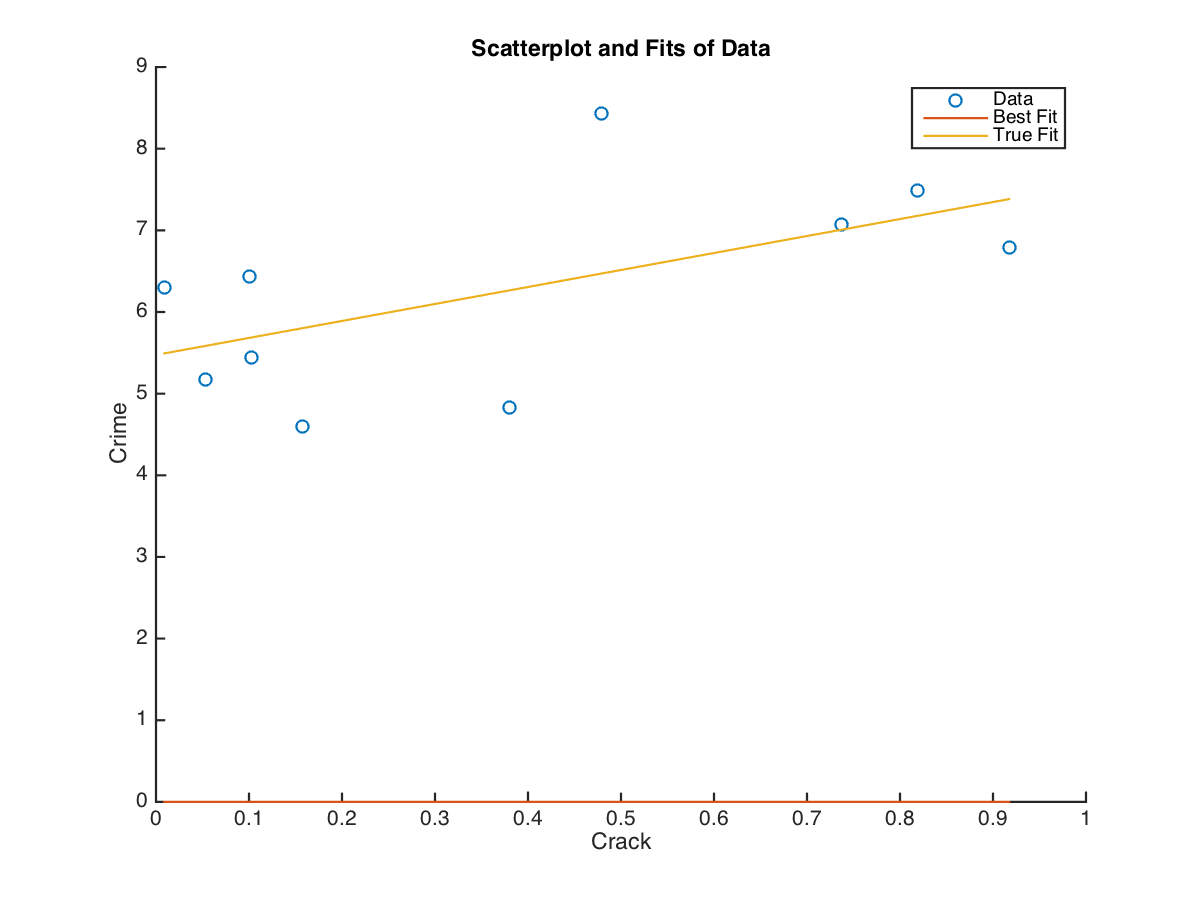
\includegraphics[scale=0.5]{Newton_OLS_Figure_1.png}
\end{figure}
\end{frame}

\begin{frame}
\frametitle[alignment=center]{Step 1}
\begin{figure}
\centering
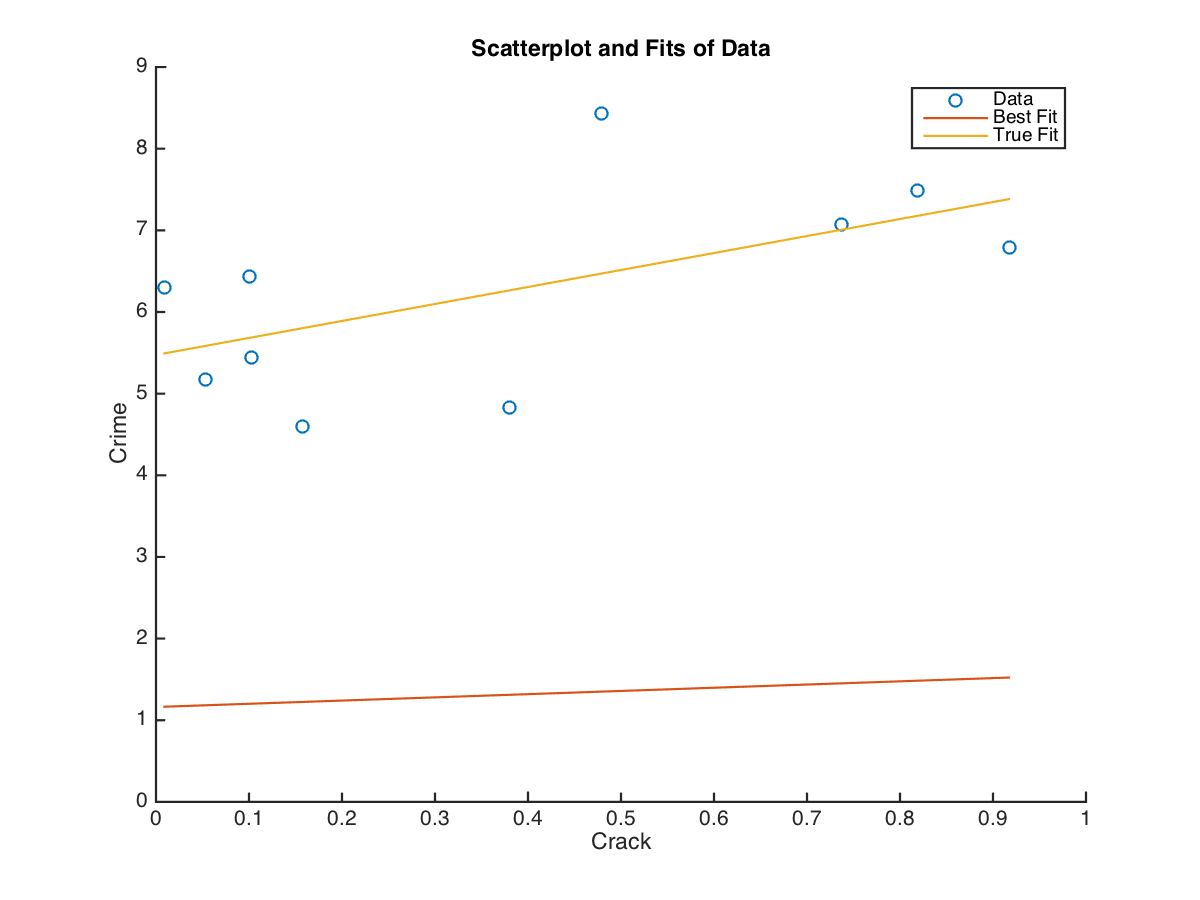
\includegraphics[scale=0.5]{Newton_OLS_Figure_2.png}
\end{figure}
\end{frame}

\begin{frame}
\frametitle[alignment=center]{...next step}
\begin{figure}
\centering
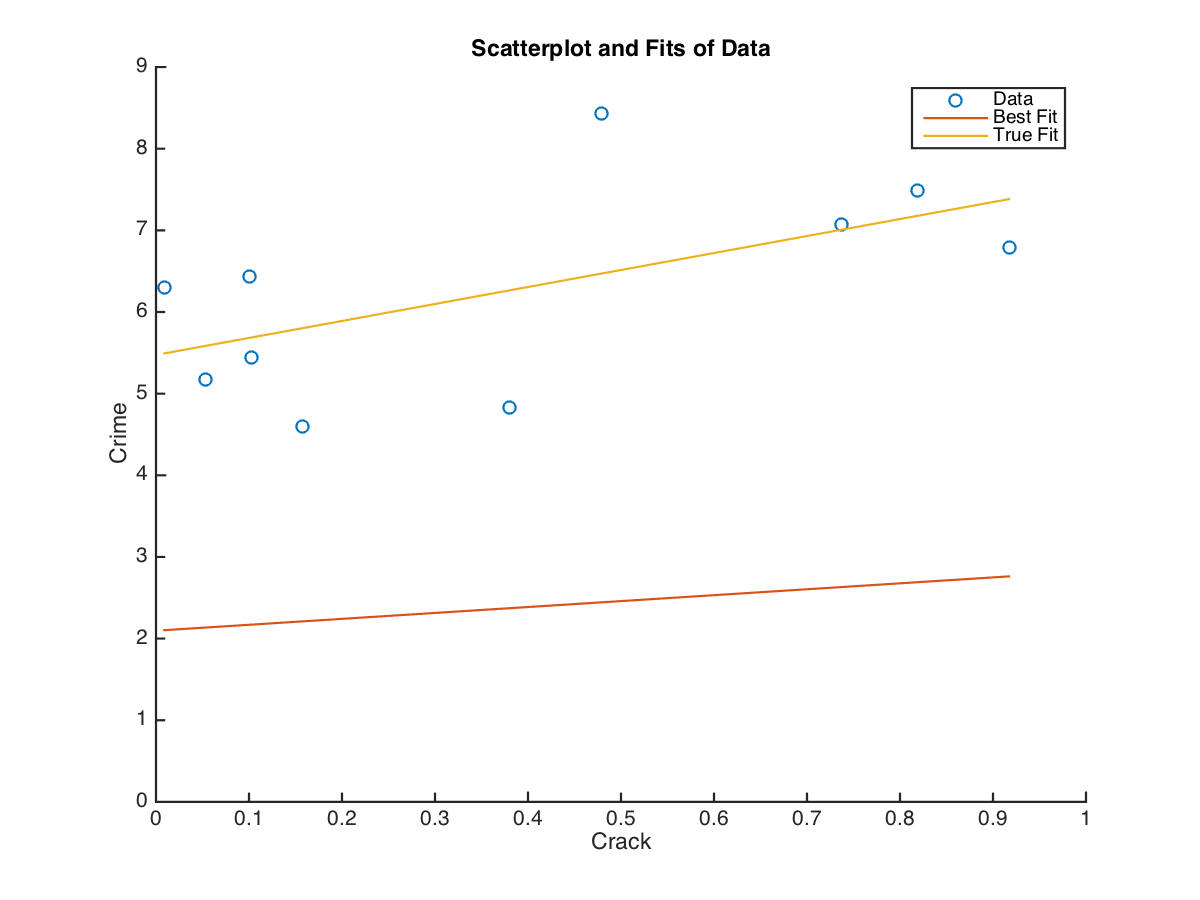
\includegraphics[scale=0.5]{Newton_OLS_Figure_3.png}
\end{figure}
\end{frame}

\begin{frame}
\frametitle[alignment=center]{...next step}
\begin{figure}
\centering
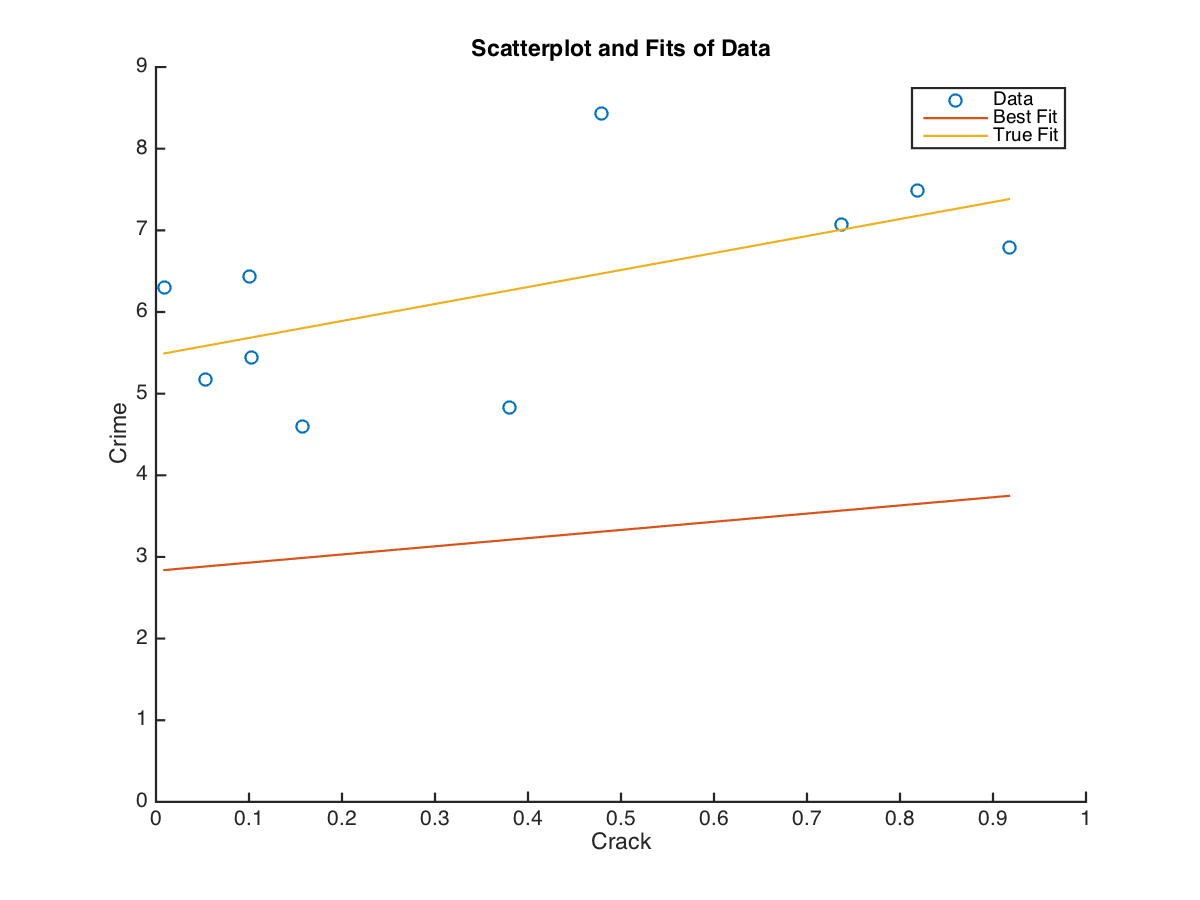
\includegraphics[scale=0.5]{Newton_OLS_Figure_4.png}
\end{figure}
\end{frame}

\begin{frame}
\frametitle[alignment=center]{...next step}
\begin{figure}
\centering
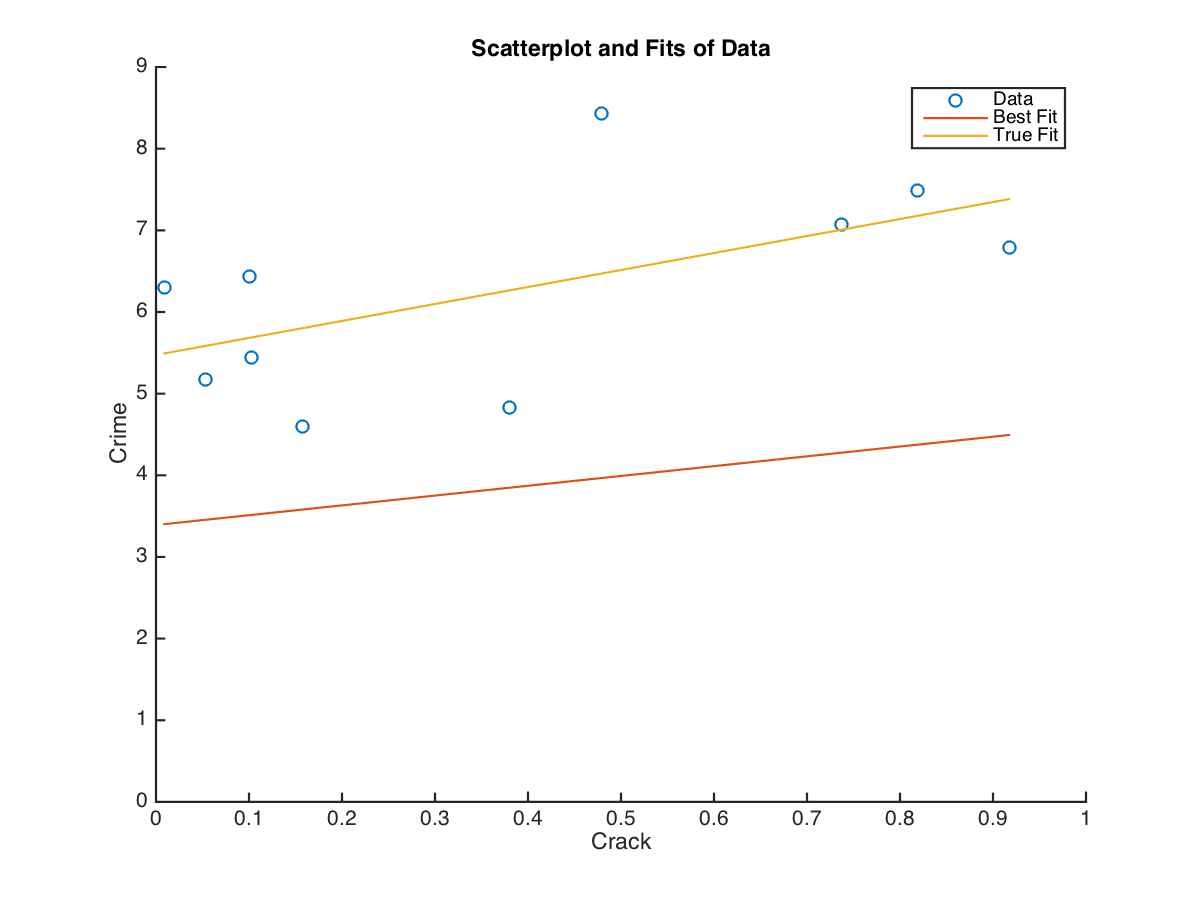
\includegraphics[scale=0.5]{Newton_OLS_Figure_5.png}
\end{figure}
\end{frame}

\begin{frame}
\frametitle[alignment=center]{...next step}
\begin{figure}
\centering
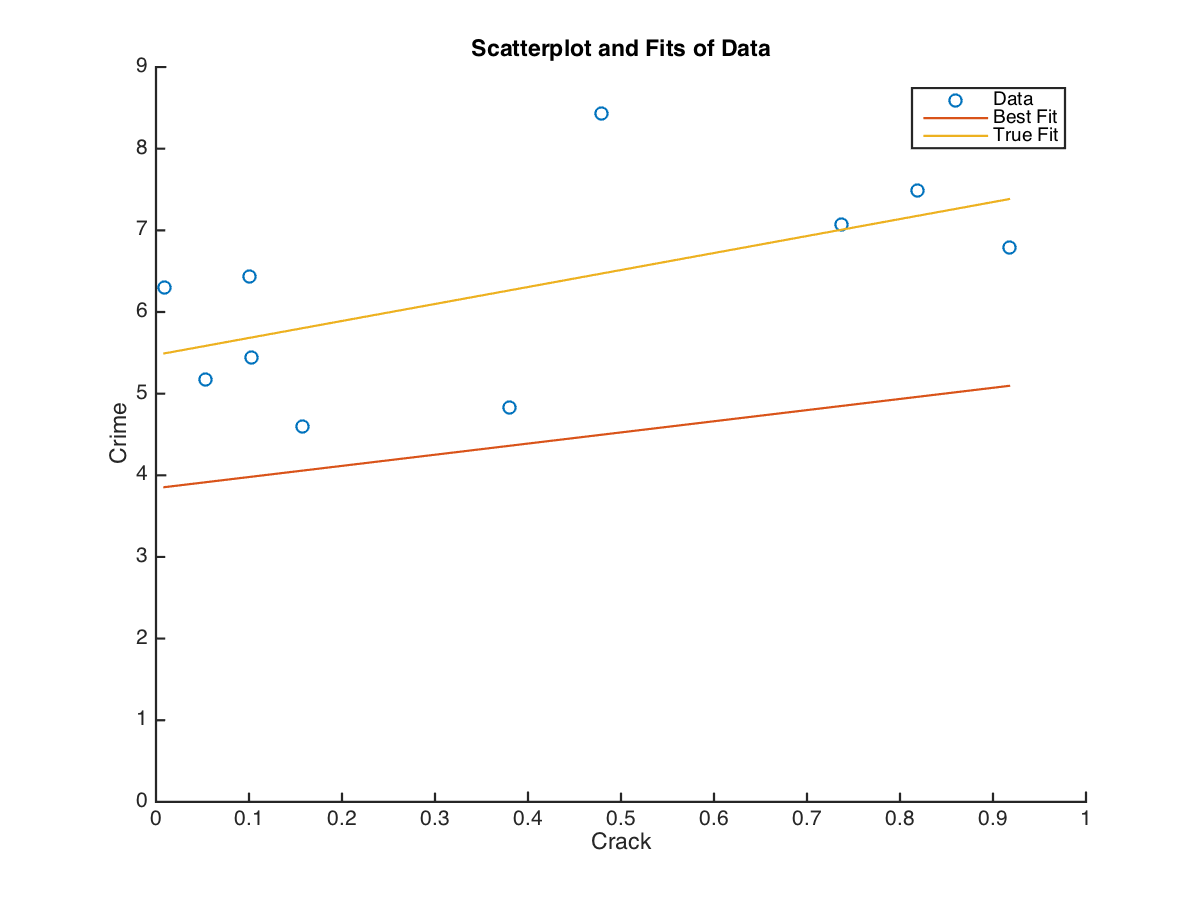
\includegraphics[scale=0.5]{Newton_OLS_Figure_6.png}
\end{figure}
\end{frame}

\begin{frame}
\frametitle[alignment=center]{...next step}
\begin{figure}
\centering
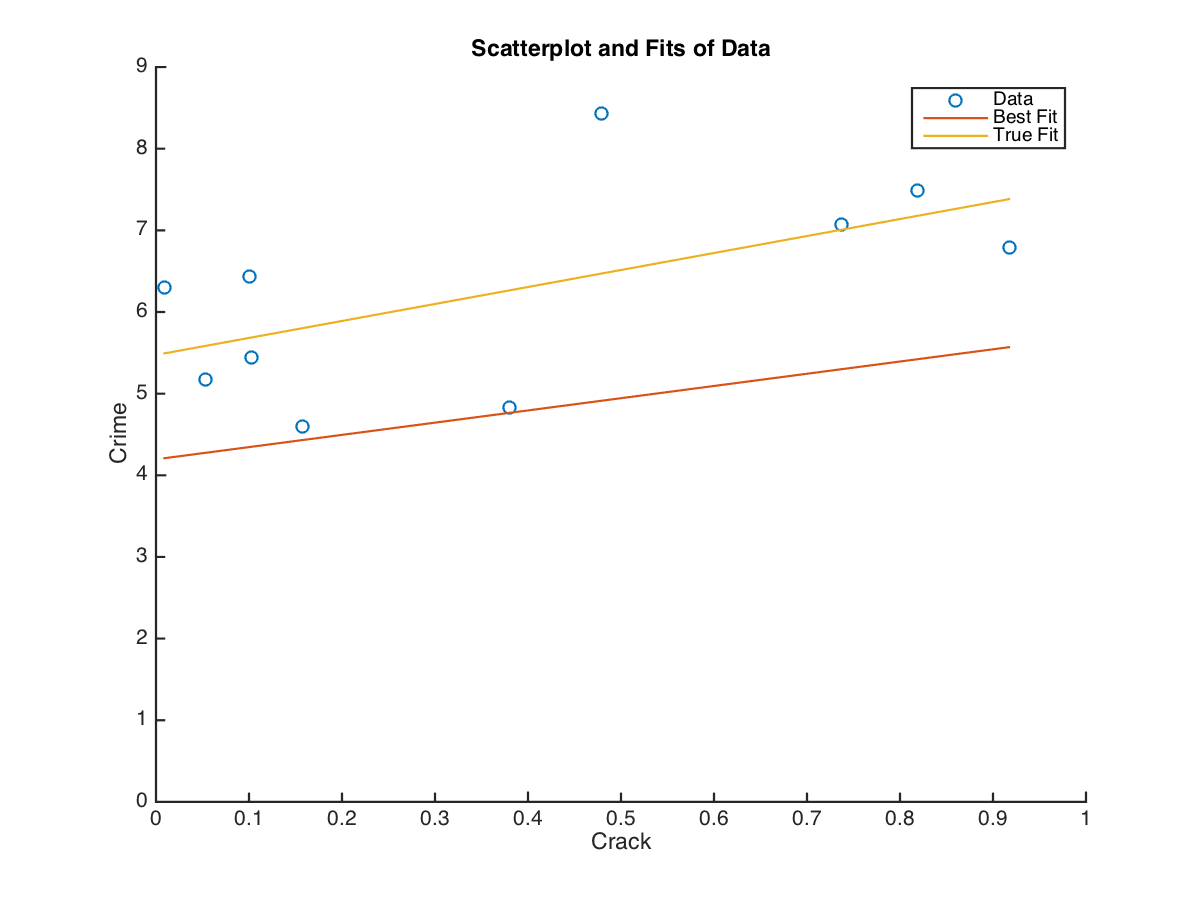
\includegraphics[scale=0.5]{Newton_OLS_Figure_7.png}
\end{figure}
\end{frame}

\begin{frame}
\frametitle[alignment=center]{...next step}
\begin{figure}
\centering
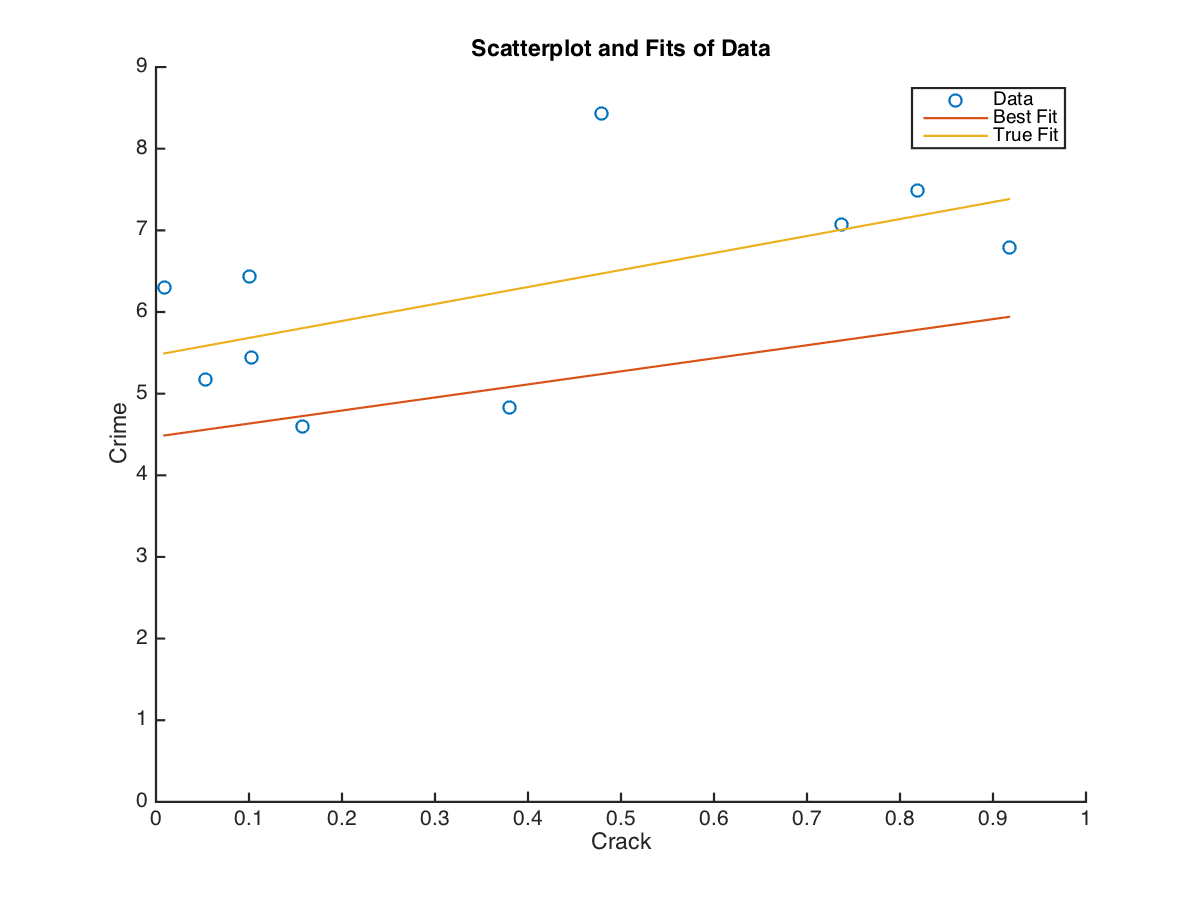
\includegraphics[scale=0.5]{Newton_OLS_Figure_8.png}
\end{figure}
\end{frame}

\begin{frame}
\frametitle[alignment=center]{...next step}
\begin{figure}
\centering
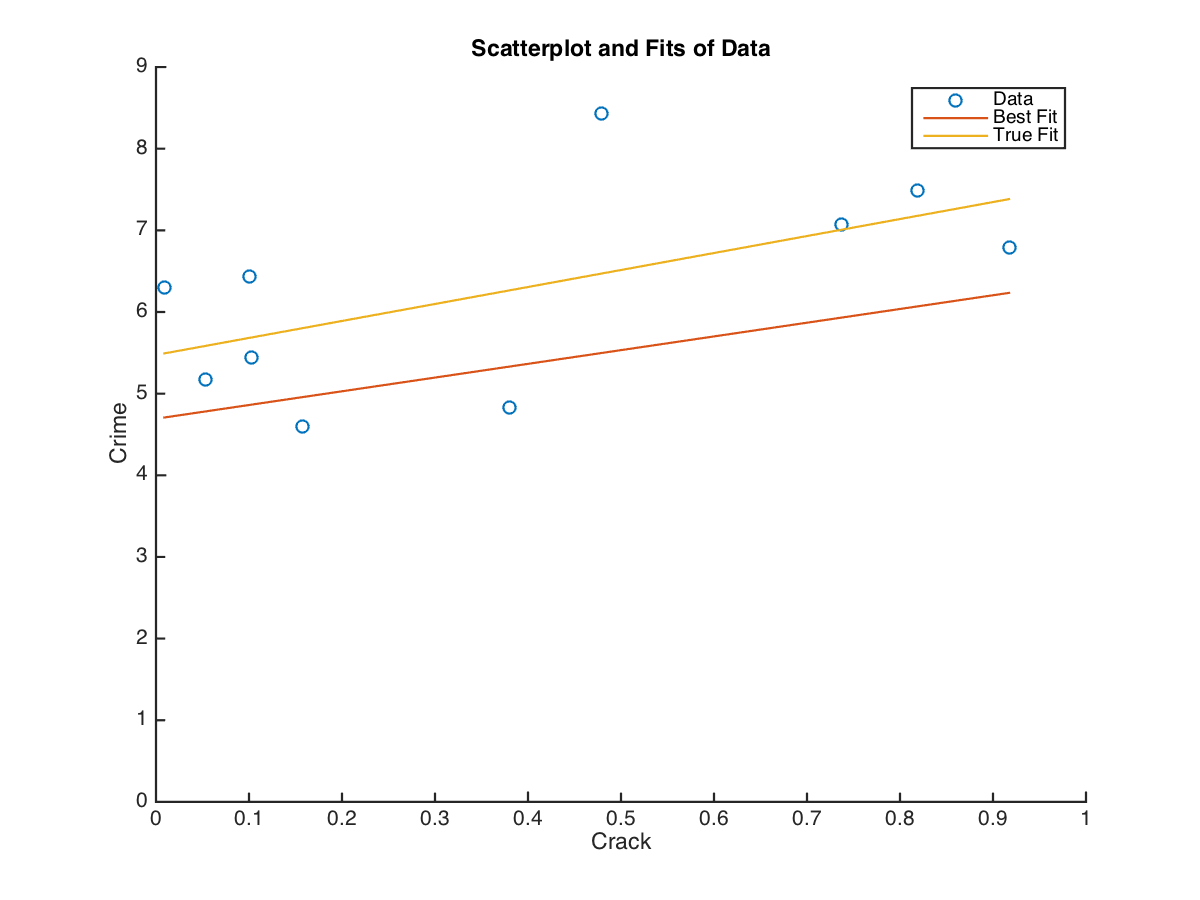
\includegraphics[scale=0.5]{Newton_OLS_Figure_9.png}
\end{figure}
\end{frame}

\begin{frame}
\frametitle[alignment=center]{...next step}
\begin{figure}
\centering
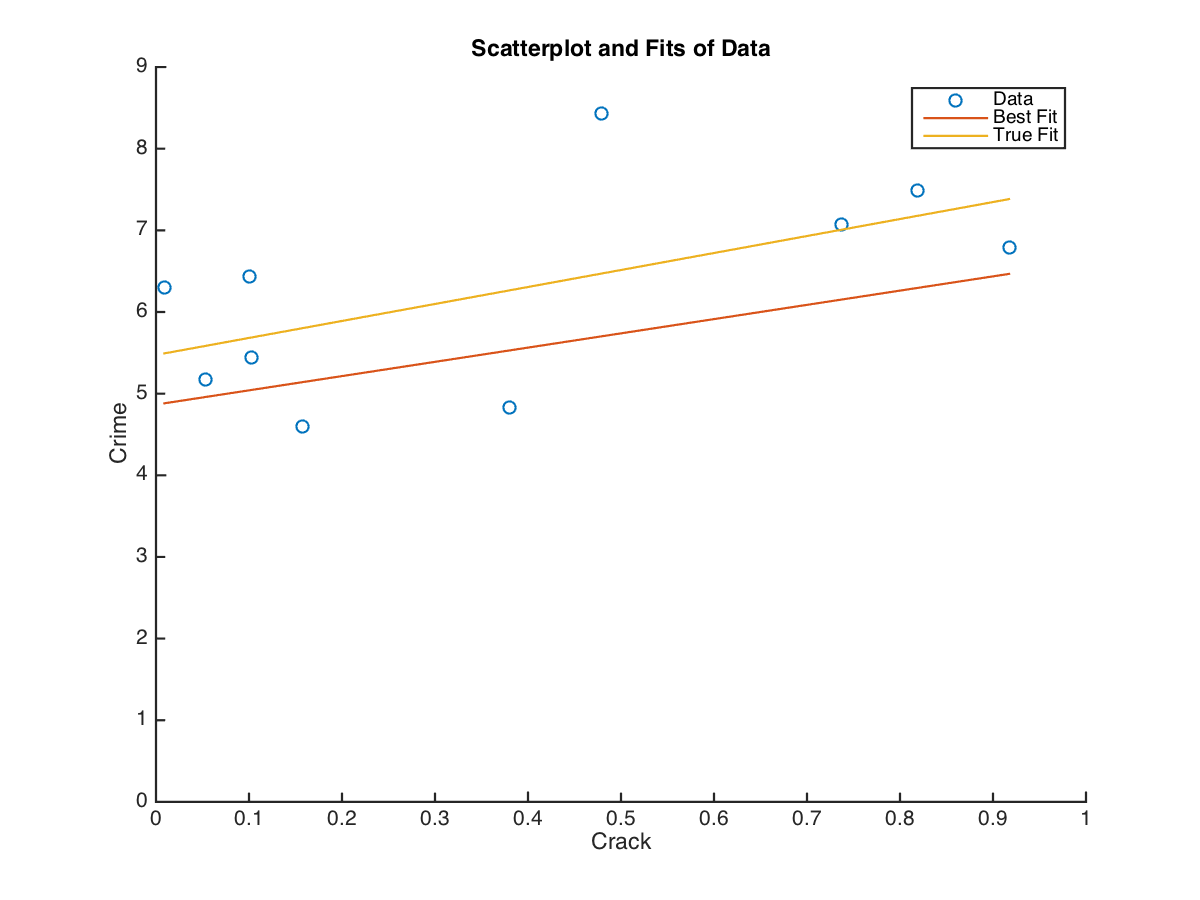
\includegraphics[scale=0.5]{Newton_OLS_Figure_10.png}
\end{figure}
\end{frame}

\begin{frame}
\frametitle[alignment=center]{...next step}
\begin{figure}
\centering
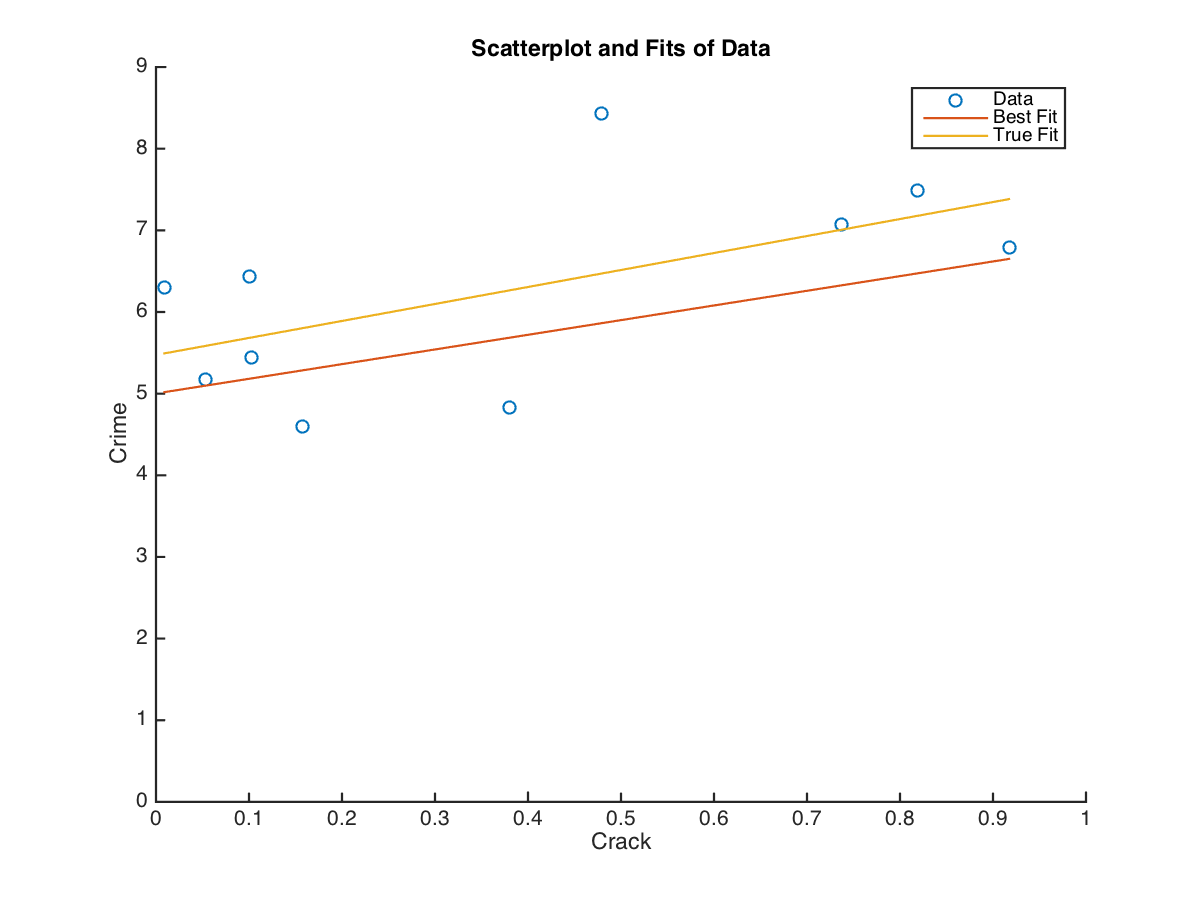
\includegraphics[scale=0.5]{Newton_OLS_Figure_11.png}
\end{figure}
\end{frame}

\begin{frame}
\frametitle[alignment=center]{...next step}
\begin{figure}
\centering
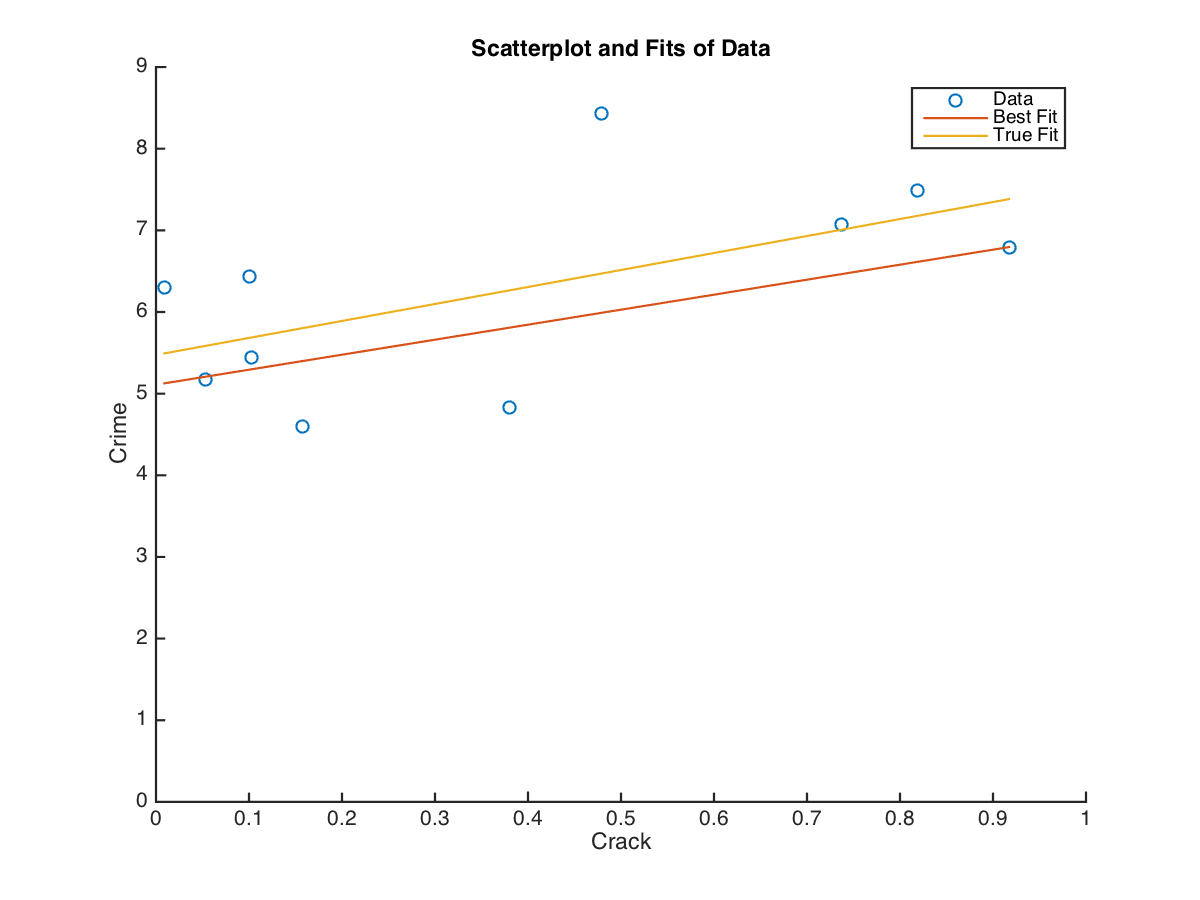
\includegraphics[scale=0.5]{Newton_OLS_Figure_12.png}
\end{figure}
\end{frame}

\begin{frame}
\frametitle[alignment=center]{...next step}
\begin{figure}
\centering
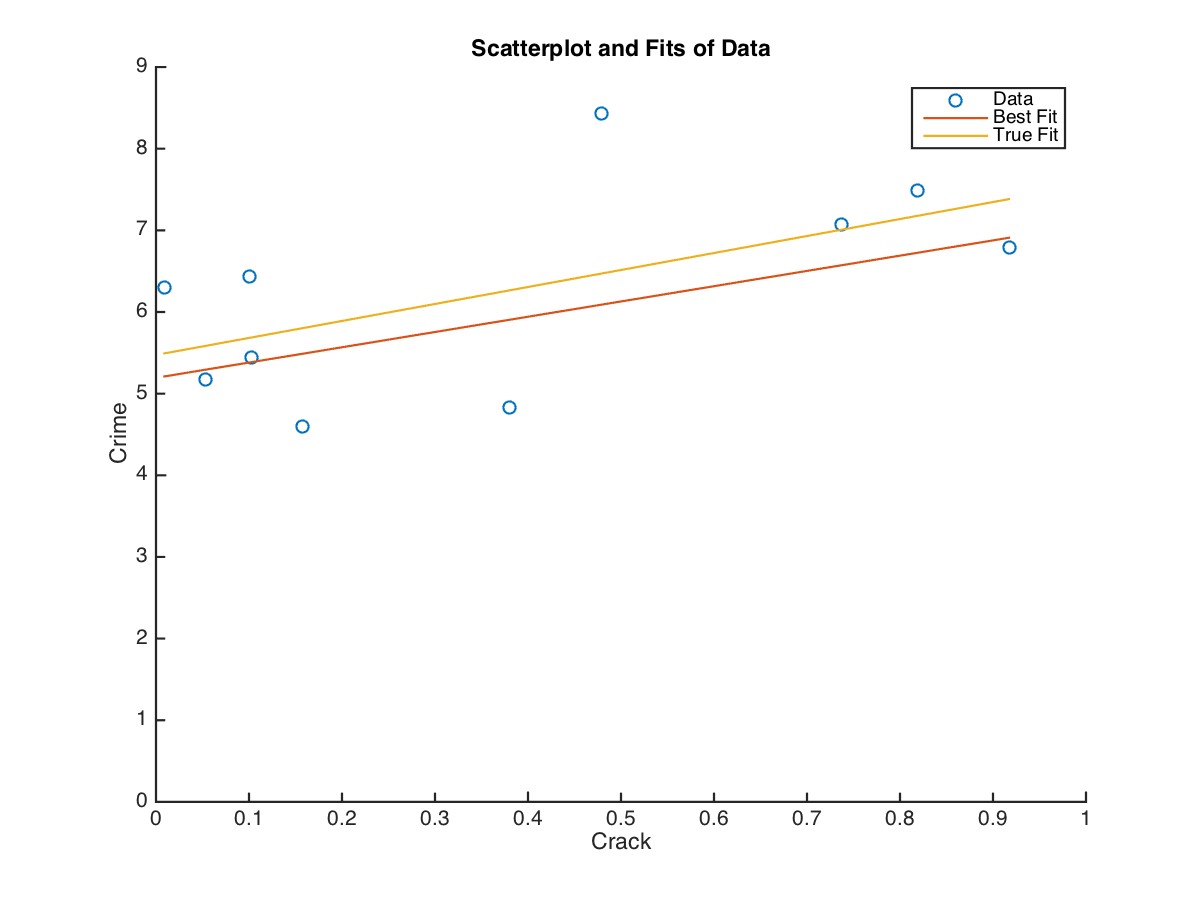
\includegraphics[scale=0.5]{Newton_OLS_Figure_13.png}
\end{figure}
\end{frame}

\begin{frame}
\frametitle[alignment=center]{...next step}
\begin{figure}
\centering
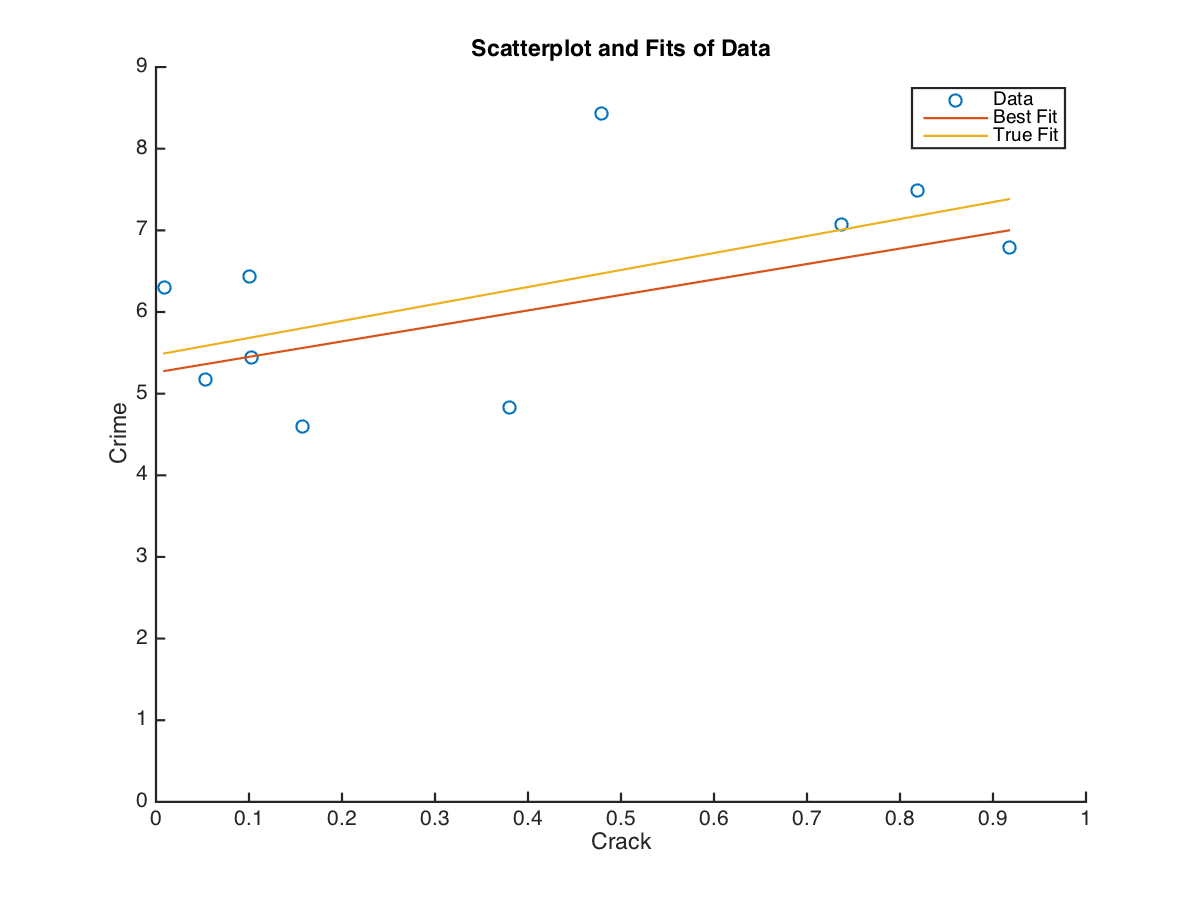
\includegraphics[scale=0.5]{Newton_OLS_Figure_14.png}
\end{figure}
\end{frame}

\begin{frame}
\frametitle[alignment=center]{...next step}
\begin{figure}
\centering
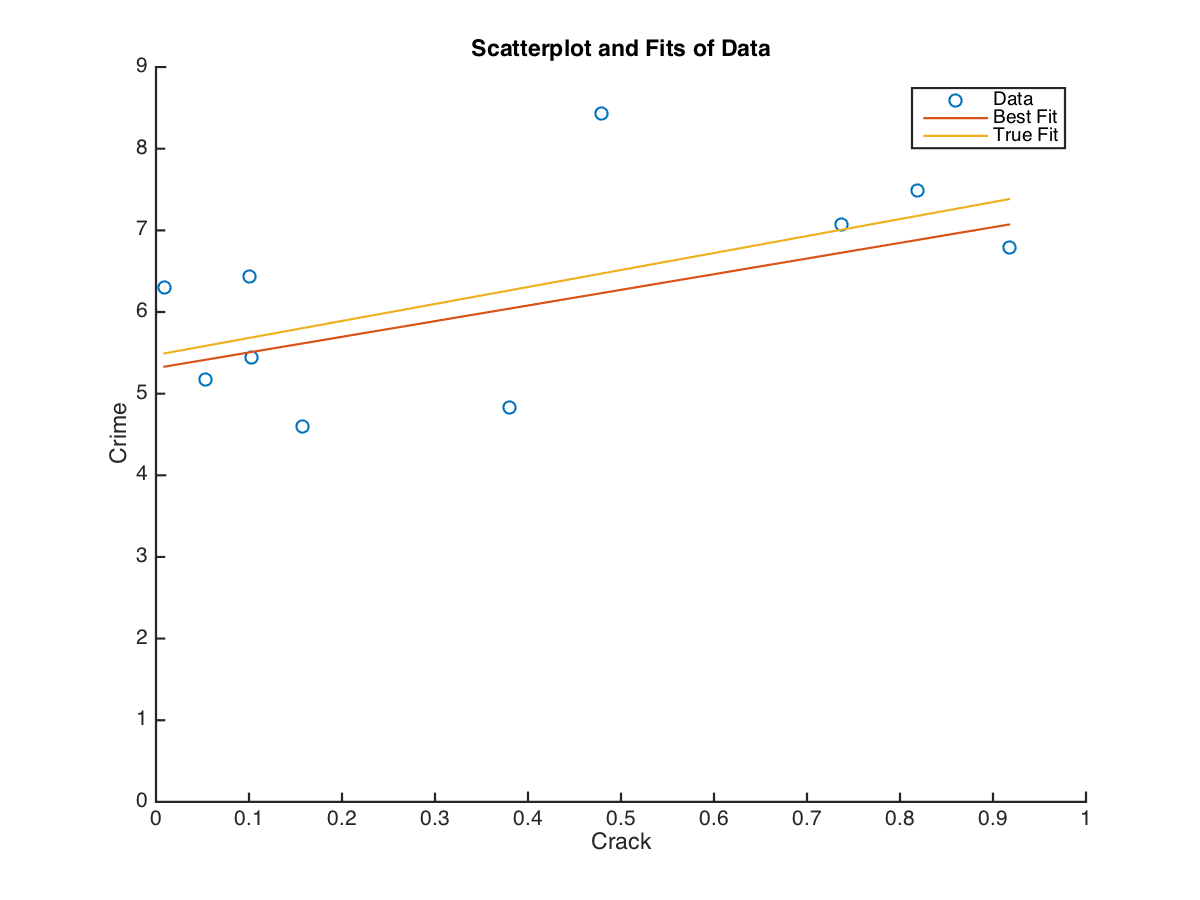
\includegraphics[scale=0.5]{Newton_OLS_Figure_15.png}
\end{figure}
\end{frame}

\begin{frame}
\frametitle[alignment=center]{...next step}
\begin{figure}
\centering
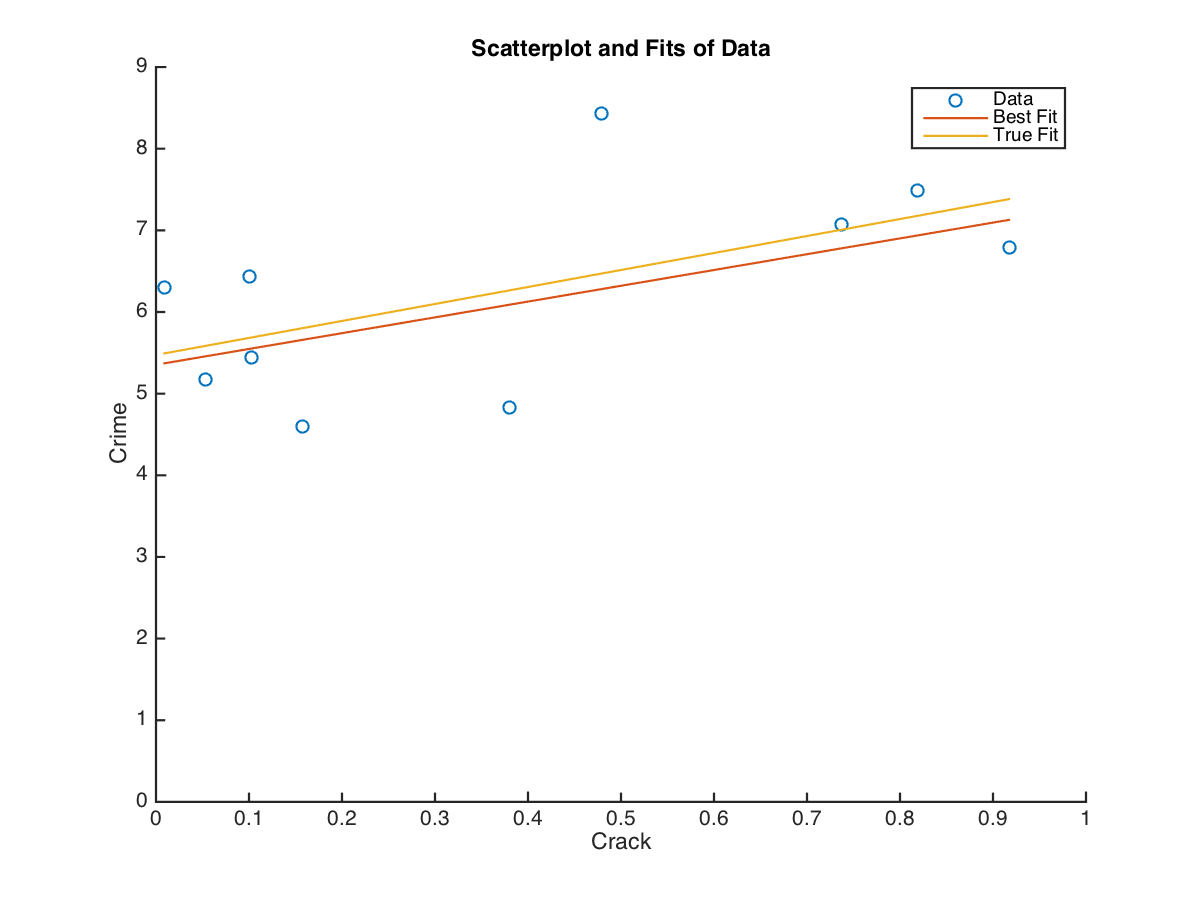
\includegraphics[scale=0.5]{Newton_OLS_Figure_16.png}
\end{figure}
\end{frame}

\begin{frame}
\frametitle[alignment=center]{...next step}
\begin{figure}
\centering
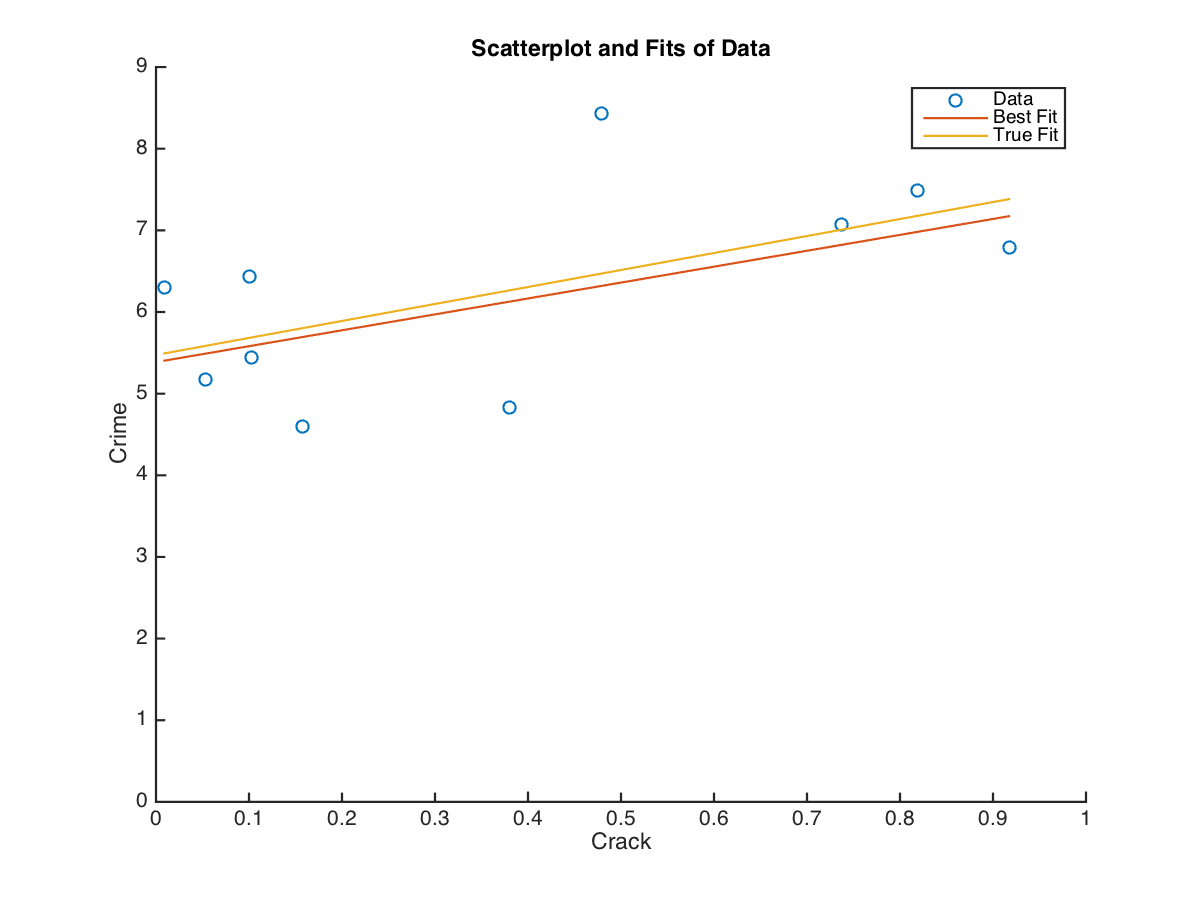
\includegraphics[scale=0.5]{Newton_OLS_Figure_17.png}
\end{figure}
\end{frame}

\begin{frame}
\frametitle[alignment=center]{...next step}
\begin{figure}
\centering
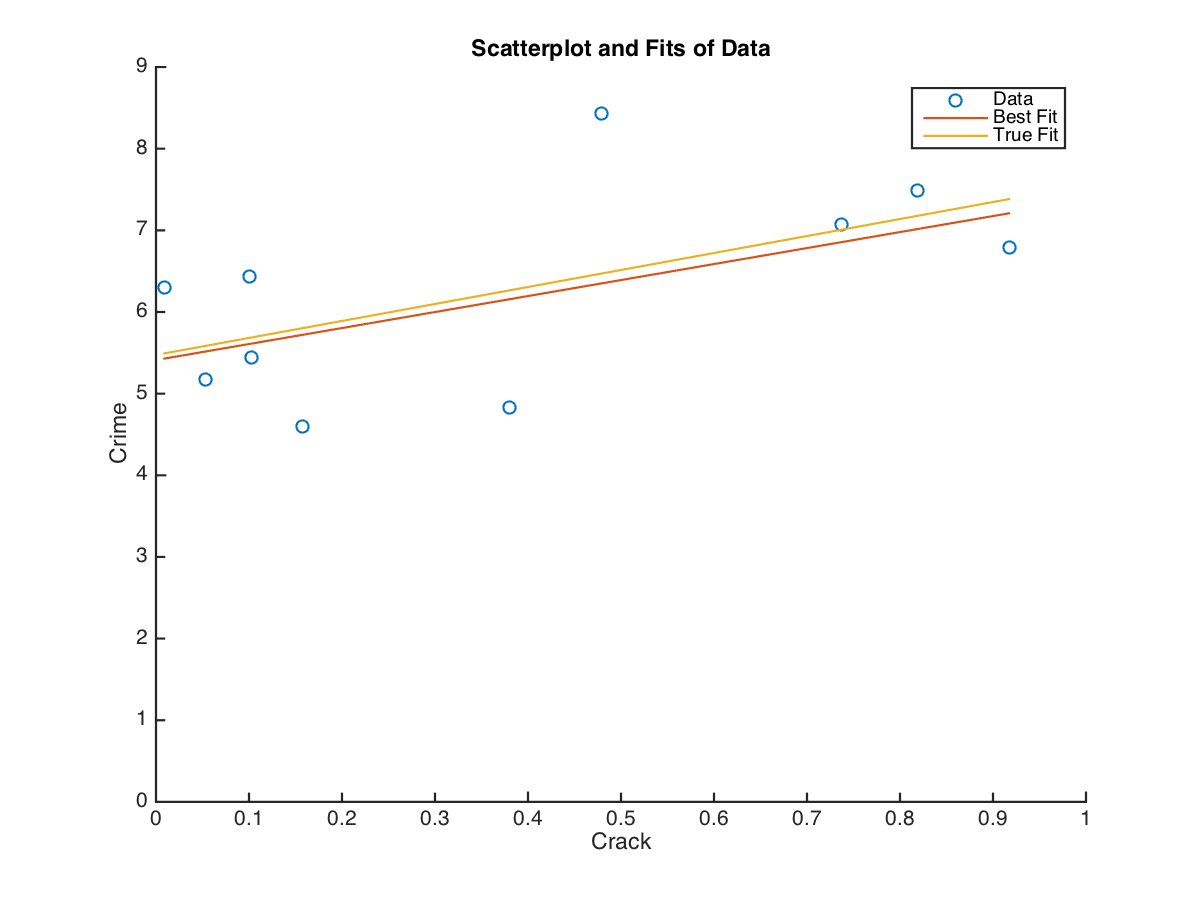
\includegraphics[scale=0.5]{Newton_OLS_Figure_18.png}
\end{figure}
\end{frame}

\begin{frame}
\frametitle[alignment=center]{...next step}
\begin{figure}
\centering
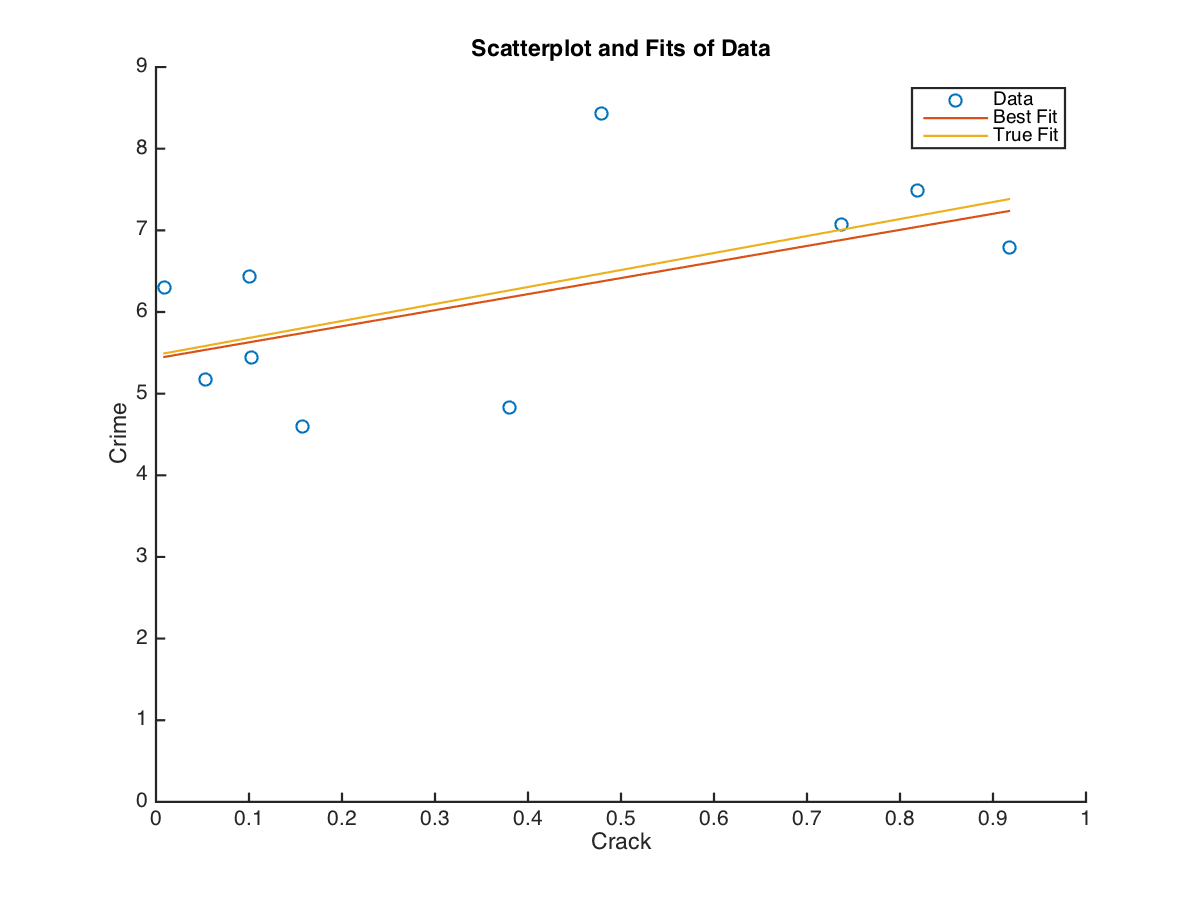
\includegraphics[scale=0.5]{Newton_OLS_Figure_19.png}
\end{figure}
\end{frame}

\begin{frame}
\frametitle[alignment=center]{...next step}
\begin{figure}
\centering
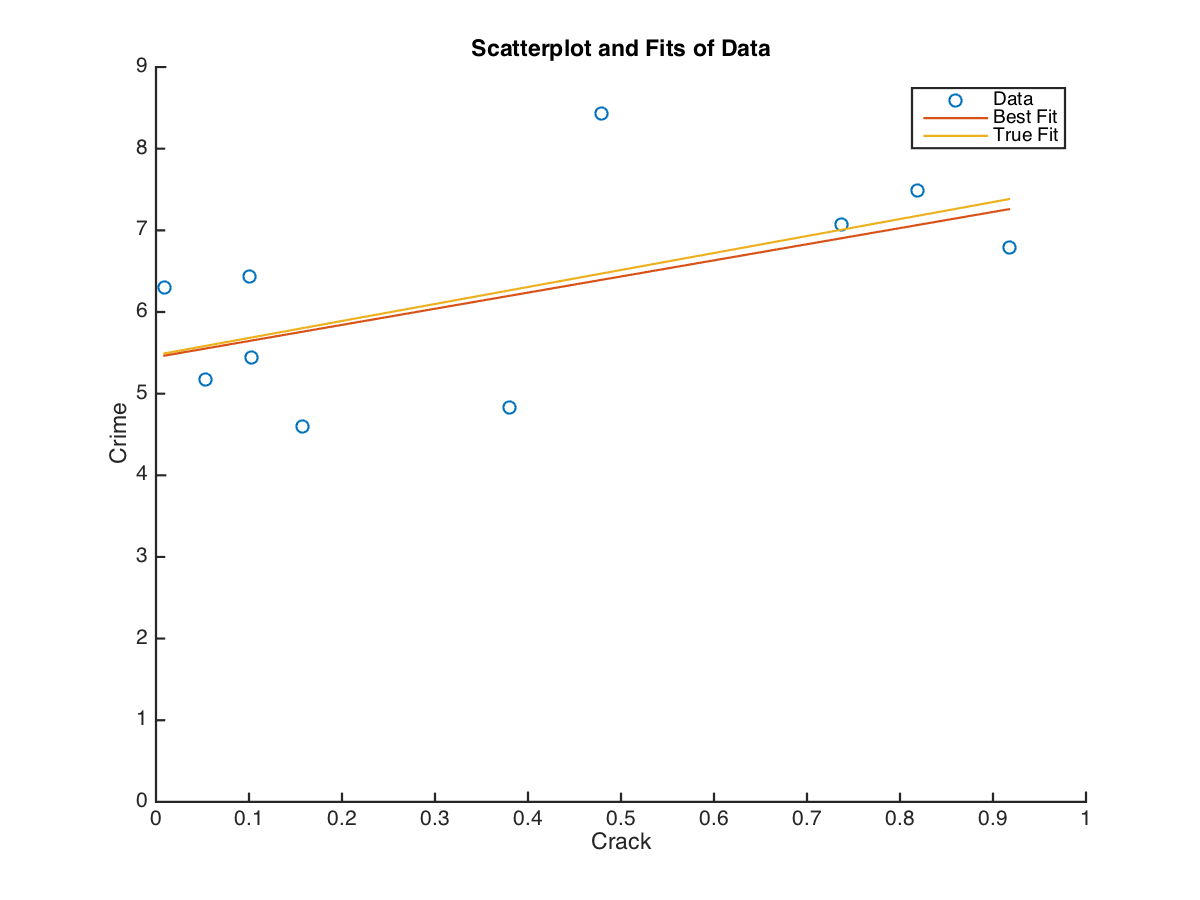
\includegraphics[scale=0.5]{Newton_OLS_Figure_20.png}
\end{figure}
\end{frame}

\begin{frame}
\frametitle[alignment=center]{...next step}
\begin{figure}
\centering
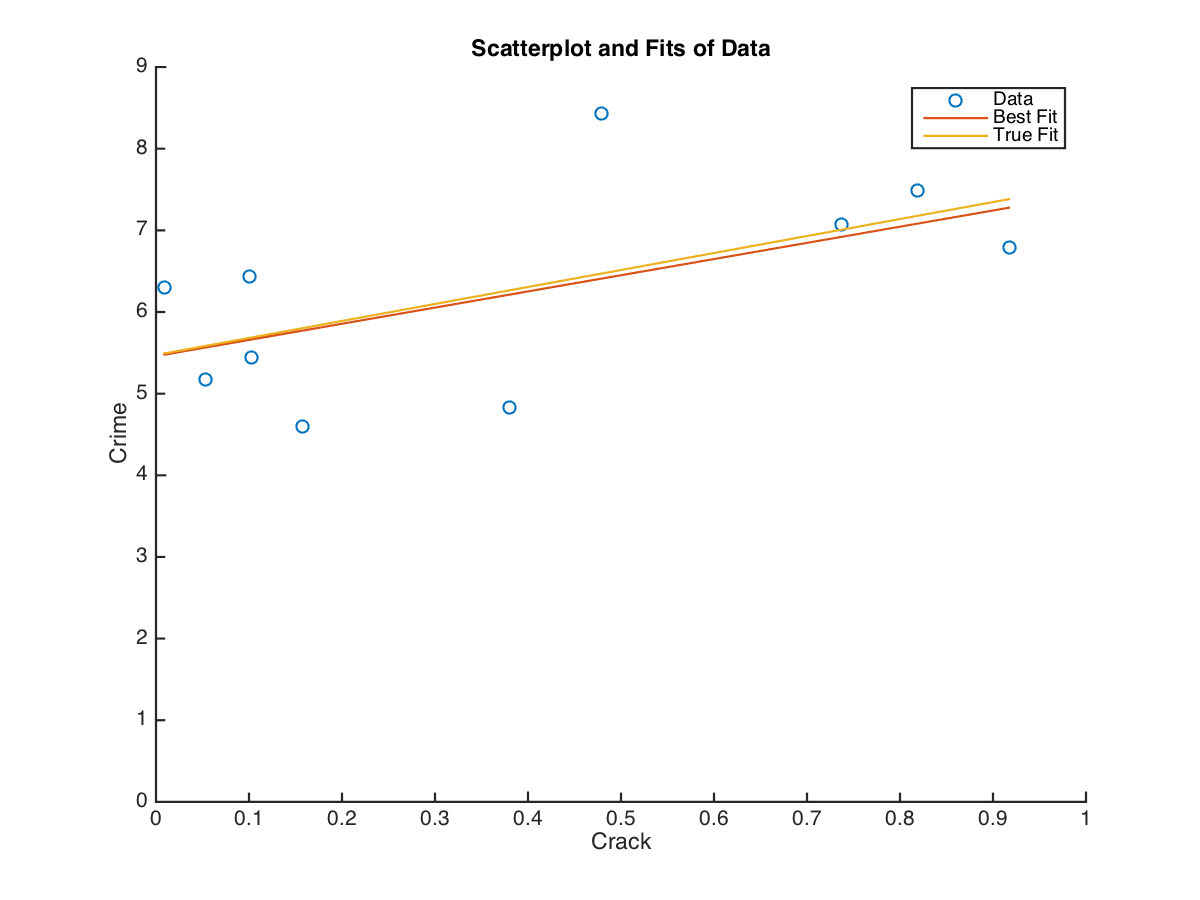
\includegraphics[scale=0.5]{Newton_OLS_Figure_21.png}
\end{figure}
\end{frame}

\begin{frame}
\frametitle[alignment=center]{...next step}
\begin{figure}
\centering
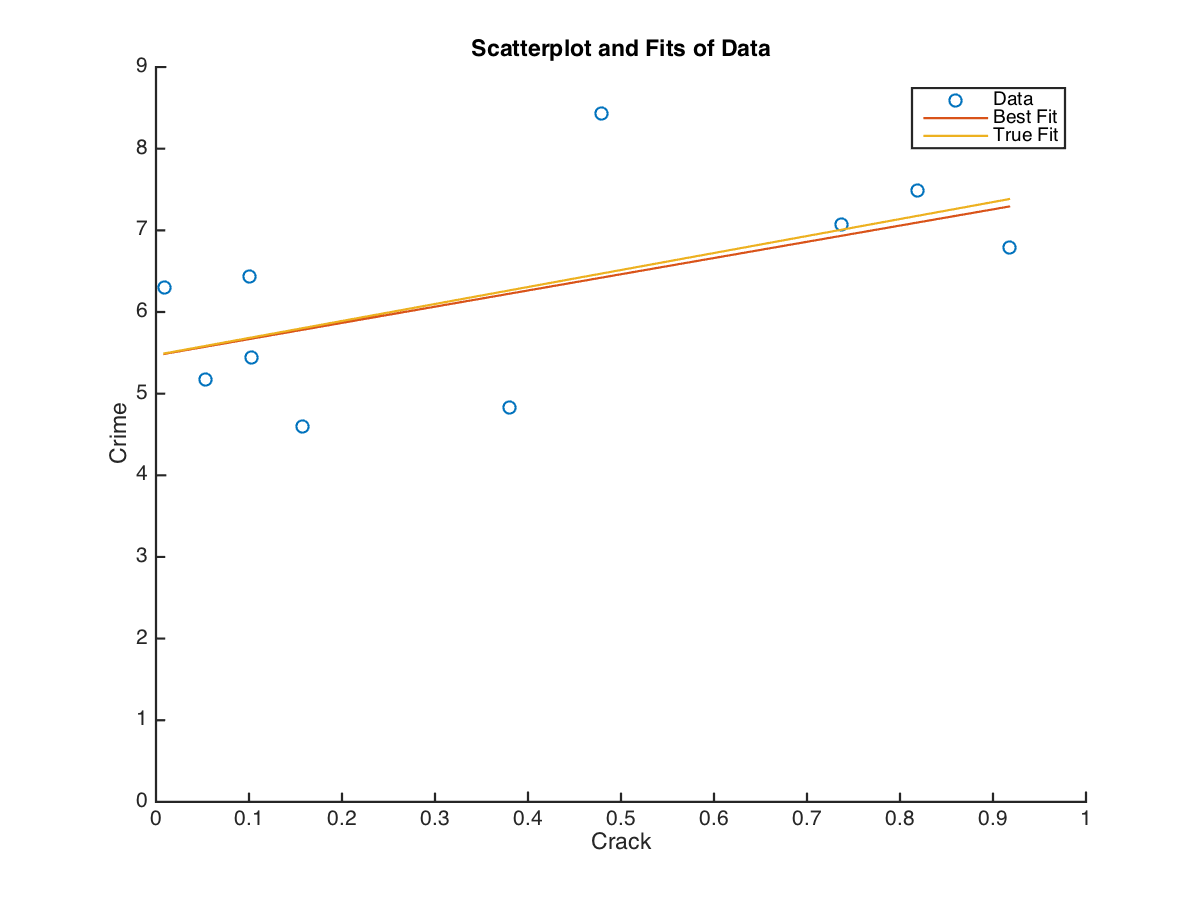
\includegraphics[scale=0.5]{Newton_OLS_Figure_22.png}
\end{figure}
\end{frame}

\begin{frame}
\frametitle[alignment=center]{...next step}
\begin{figure}
\centering
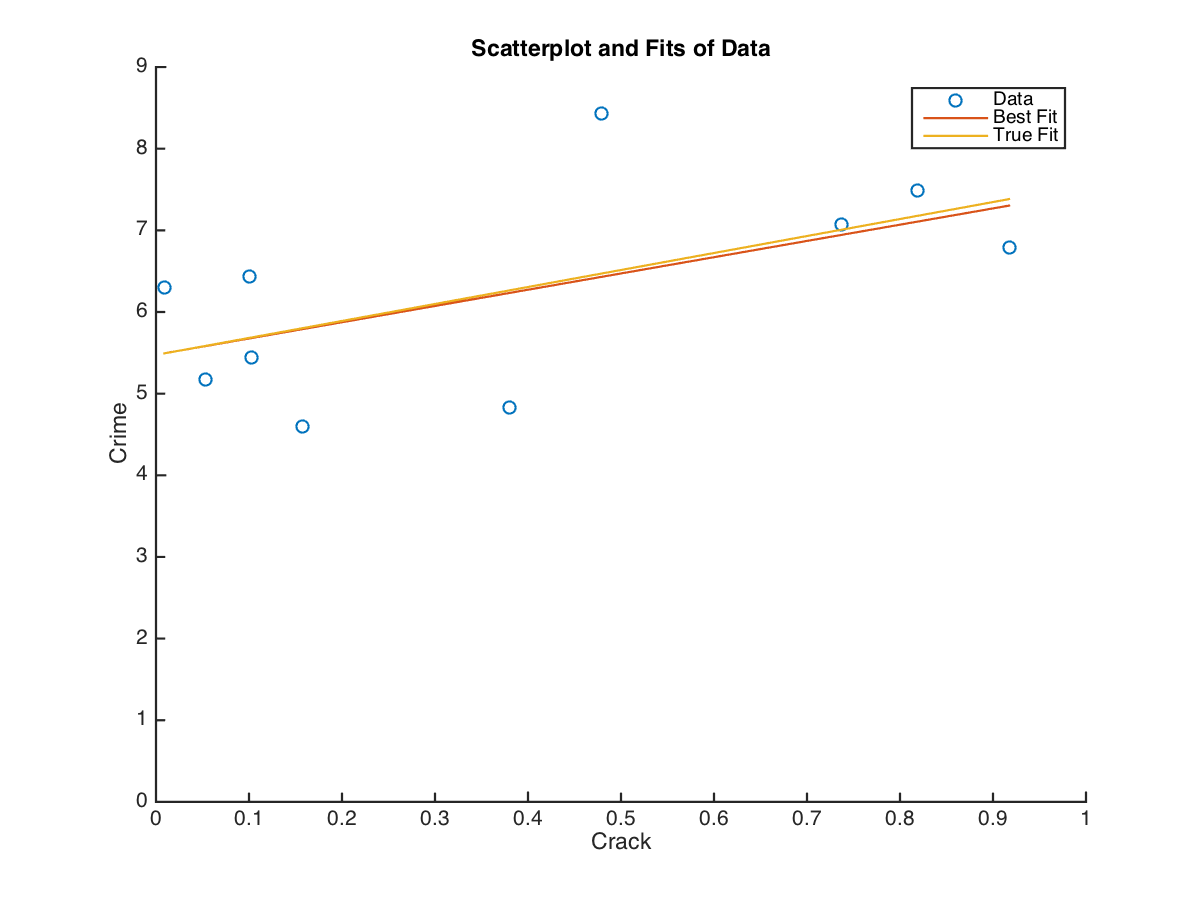
\includegraphics[scale=0.5]{Newton_OLS_Figure_23.png}
\end{figure}
\end{frame}

\begin{frame}
\frametitle[alignment=center]{...next step}
\begin{figure}
\centering
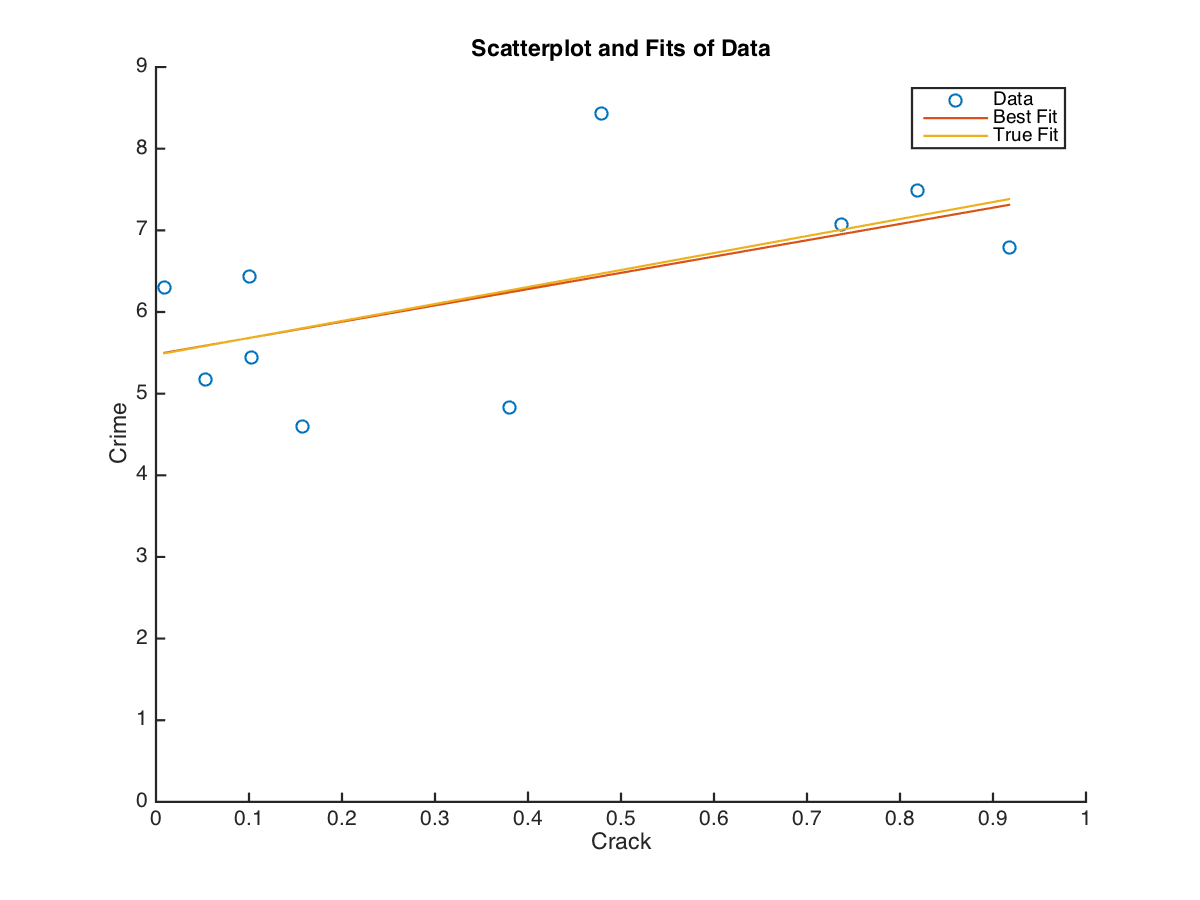
\includegraphics[scale=0.5]{Newton_OLS_Figure_24.png}
\end{figure}
\end{frame}

\begin{frame}
\frametitle[alignment=center]{...next step}
\begin{figure}
\centering
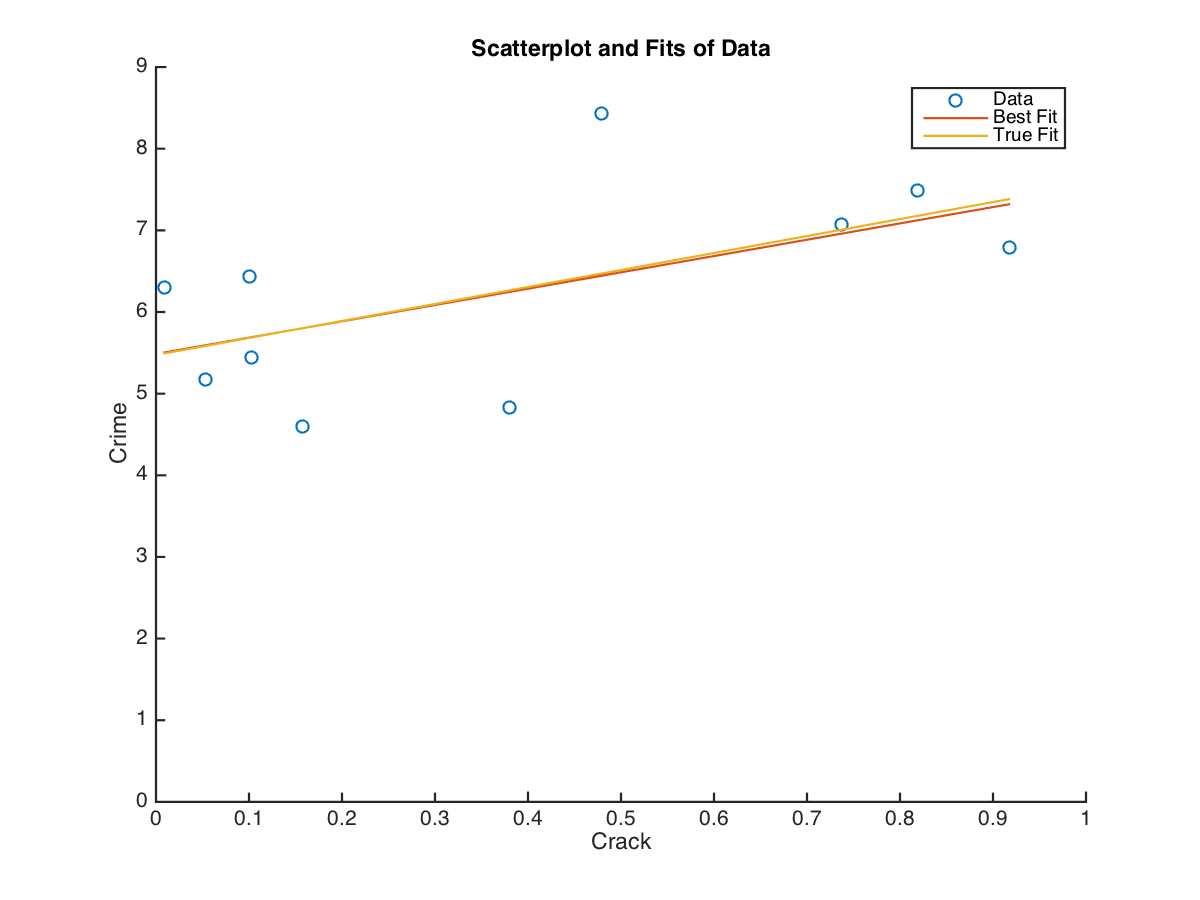
\includegraphics[scale=0.5]{Newton_OLS_Figure_25.png}
\end{figure}
\end{frame}

\begin{frame}
\frametitle[alignment=center]{...next step}
\begin{figure}
\centering
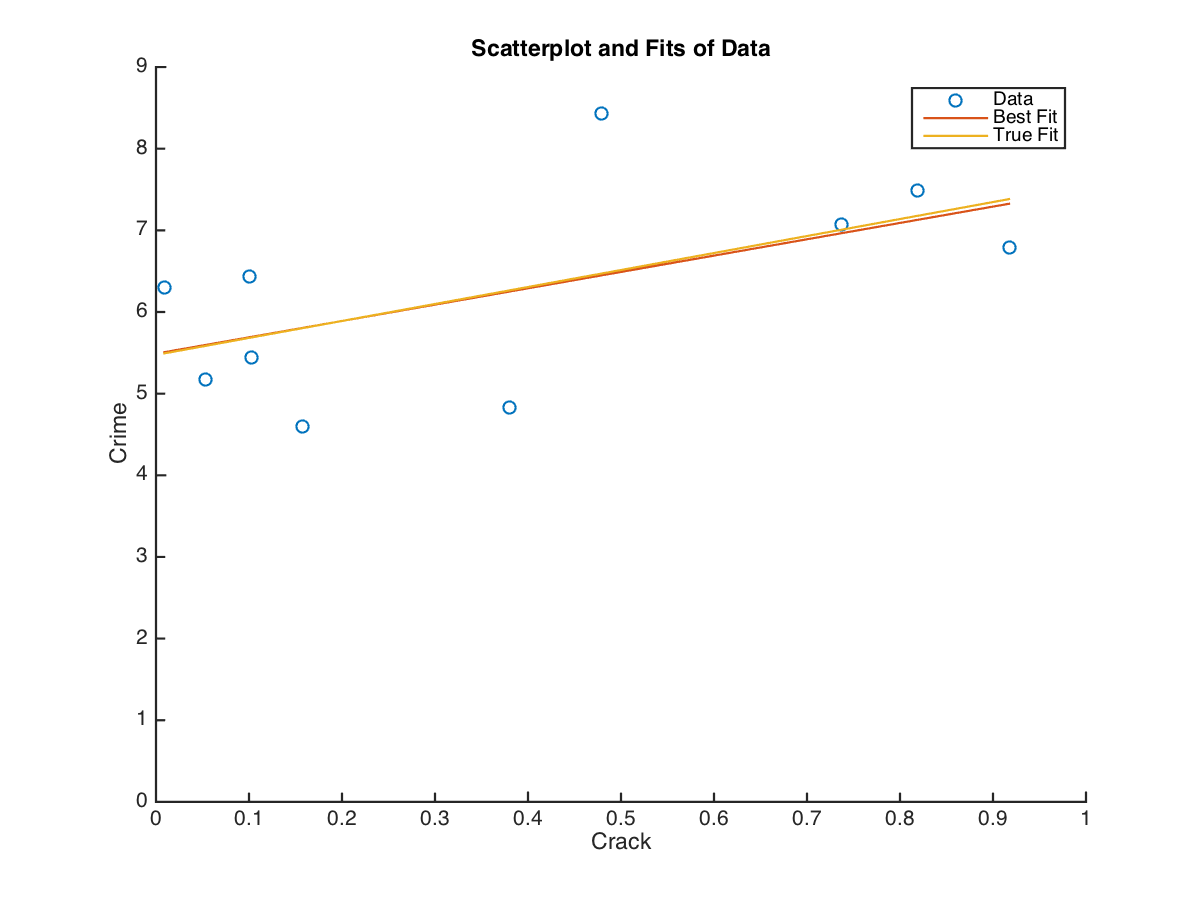
\includegraphics[scale=0.5]{Newton_OLS_Figure_26.png}
\end{figure}
\end{frame}

\begin{frame}
\frametitle[alignment=center]{...next step}
\begin{figure}
\centering
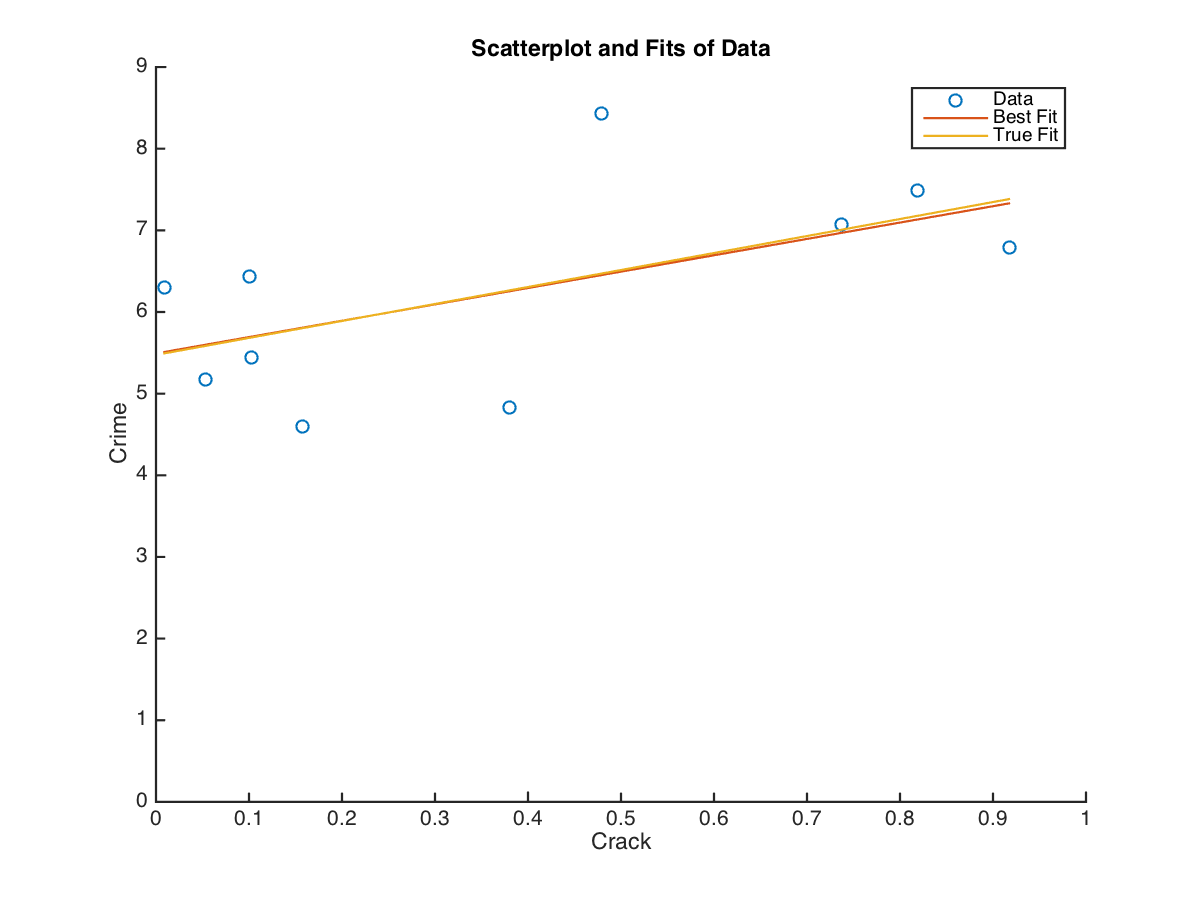
\includegraphics[scale=0.5]{Newton_OLS_Figure_27.png}
\end{figure}
\end{frame}

\begin{frame}
\frametitle[alignment=center]{...next step}
\begin{figure}
\centering
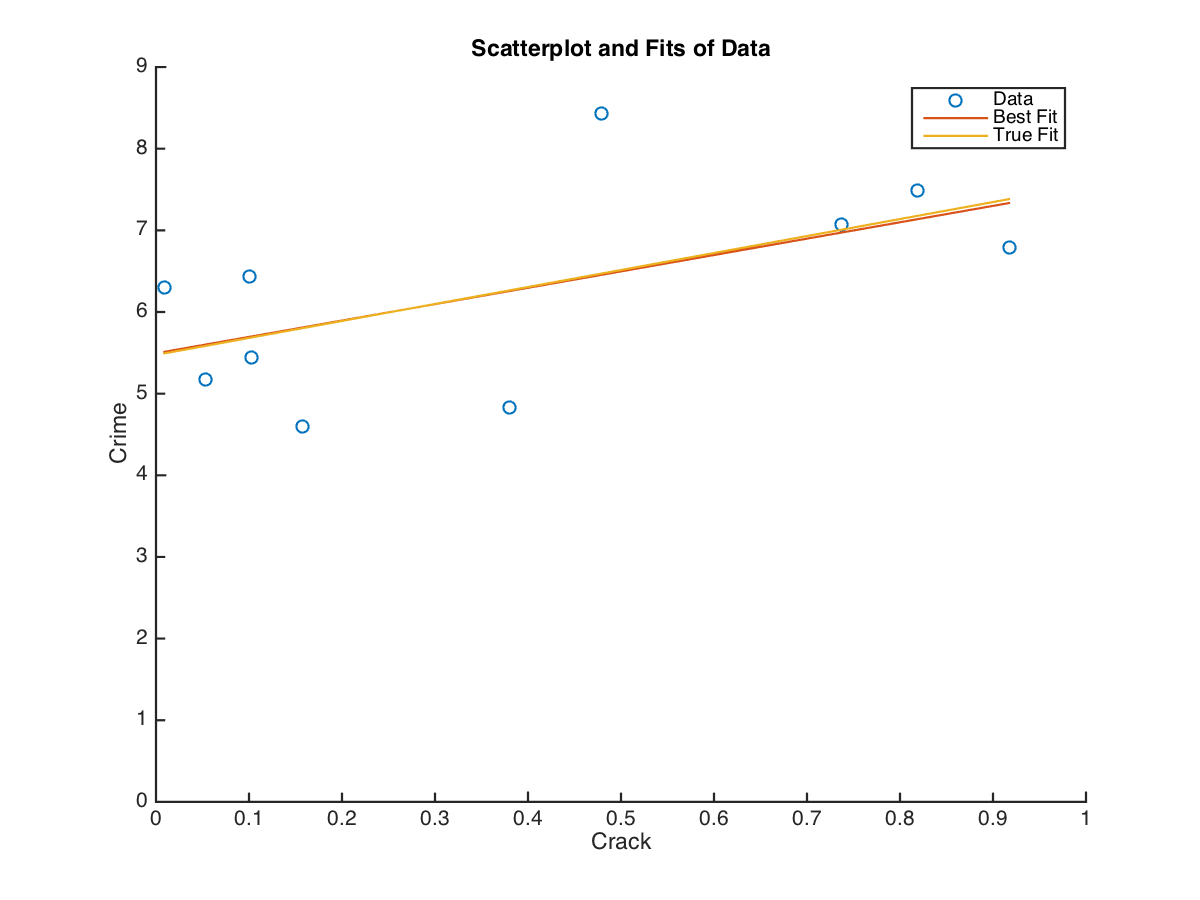
\includegraphics[scale=0.5]{Newton_OLS_Figure_28.png}
\end{figure}
\end{frame}

\begin{frame}
\frametitle[alignment=center]{28th step...}
\begin{figure}
\centering
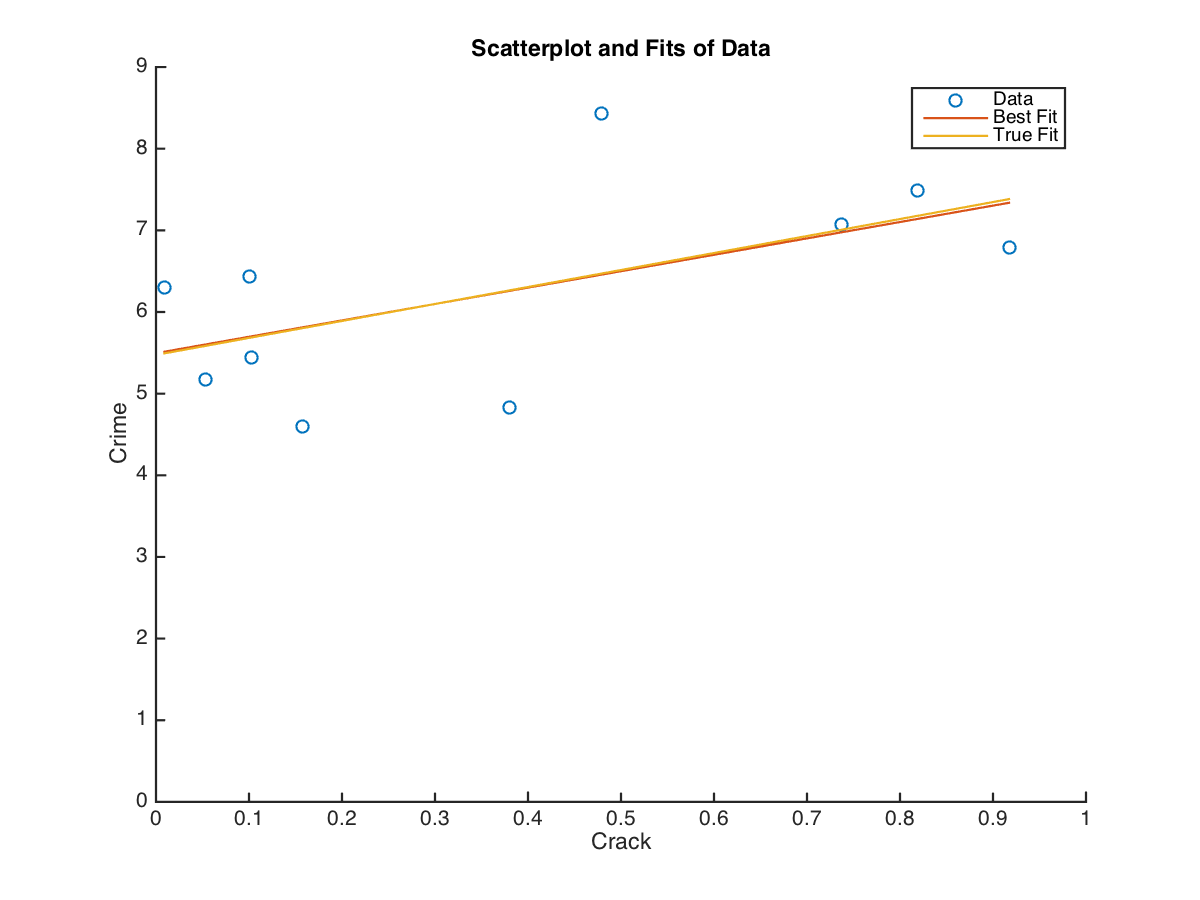
\includegraphics[scale=0.5]{Newton_OLS_Figure_29.png}
\end{figure}
\end{frame}

\begin{frame}
\frametitle[alignment=center]{Last step!}
\begin{figure}
\centering
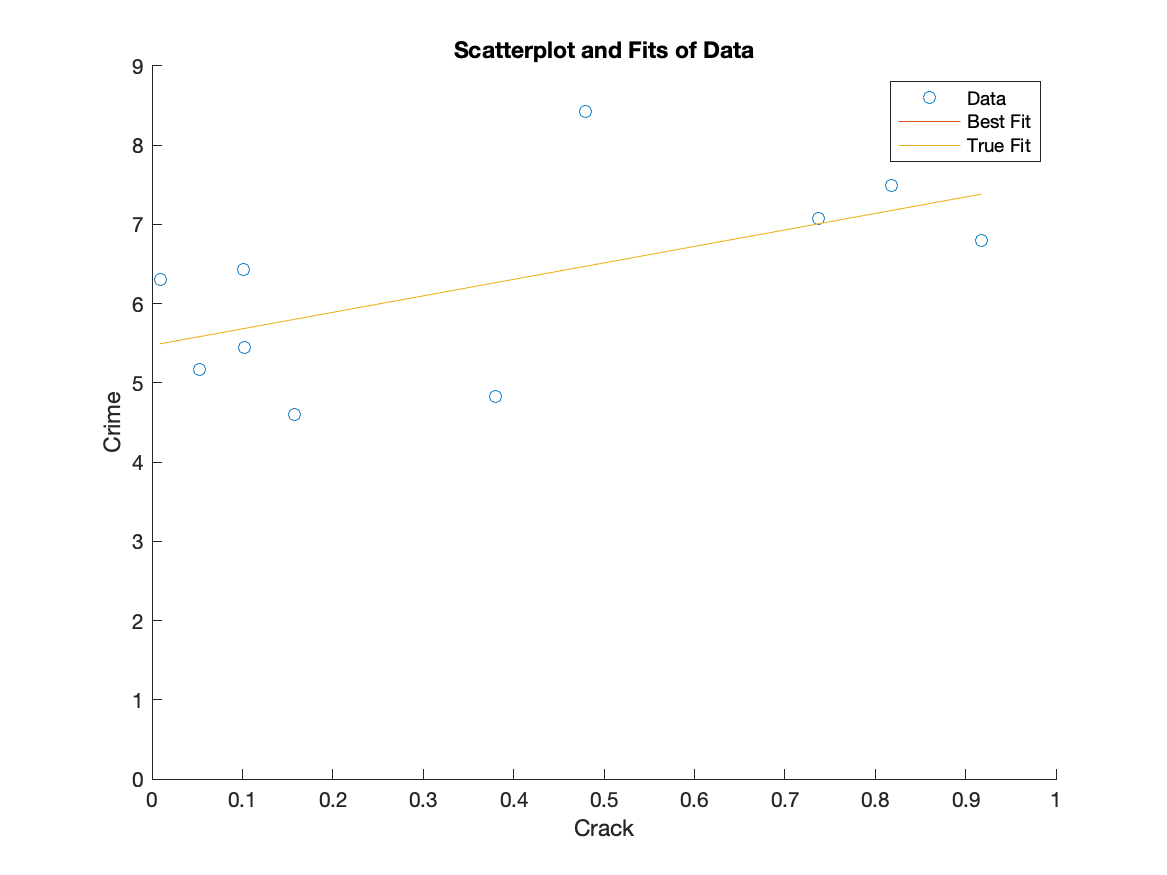
\includegraphics[scale=0.5]{Newton_OLS_Figure_30.png}
\end{figure}
Note: took about 863 steps to get both gradients to $<10^{-10}$.
\end{frame}


%\begin{frame}
%\frametitle[alignment=center]{In Matlab}
%\begin{itemize}
%%Then we can do newton's method easily:
%\end{itemize}
%\end{frame}


\end{document}